\documentclass{sprawozdanie-agh}


\usepackage[utf8]{inputenc}
\usepackage{listings}
\usepackage{pdfpages}
\usepackage{float}
\usepackage{anyfontsize}
\usepackage{courier}
\usepackage{hyperref}

\lstset{basicstyle=\footnotesize\ttfamily,breaklines=true}
 
\makeatletter 

\begin{document}   

	\przedmiot{Inżynieria oprogramowania}
	\tytul{Dokumentacja}
	\podtytul{„Gdzie jest moje dziecko?”}
	\kierunek{Informatyka, III rok, 2018/2019}
	\autor{Agnieszka Zadworny, Piotr Morawiecki, Tomasz Pęcak, Maciej Bielech}
	\data{Kraków, 7 listopada 2018}

	\stronatytulowa{}

	

	\section{Jak zbudować i uruchomić aplikację webową na "devie"?}

		\subsection{Potrzebne pliki}

			Do poprawnego działania aplikacji potrzebujemy dwóch plików, które nie są udostępnione w repozytorium z uwagi na bezpieczeństwo kluczy prywatnych.
			Są to: \lstinline{/server/config/dev.js} i \lstinline{/server/client/.env.development}.
			 \begin{itemize}
				 \item \lstinline{/server/config/dev.js} zawiera: 
					\begin{lstlisting}
						module.exports = {
							googleClientID: 'googleClientID',
							googleClientSecret: 'googleClientSecret',
							mongoURI: 'mongoDBuri',
							cookieKey: 'cookieKey'
						};
					\end{lstlisting}
				\item \lstinline{/server/client/.env.development} zawiera:
					\begin{lstlisting}
						REACT_APP_GOOGLE_KEY='keyGoogleMapsAPI'
					\end{lstlisting}
			 \end{itemize}

		\subsection{Budowanie i uruchamianie}

		Aby uruchomić aplikację webową musimy pobrać pliki z repozytorium,
		nastepnie zainstalować Node.js. Aby zainstalować Node.js postępujemy według instrukcji na oficjalnej stronie nodejs.org. Przykładowe kroki dla Ubuntu i wersji 11 Node.js:

		\begin{lstlisting}
			curl -sL https://deb.nodesource.com/setup_11.x | sudo -E bash -
			sudo apt-get install -y nodejs
		\end{lstlisting}
		Kolejnym krokiem jest przejście do folderu \lstinline{/server} w projekcie i zainstalowanie potrzebnych bibliotek, uruchamiając następującą instrukcję:
		\begin{lstlisting}
			npm install
		\end{lstlisting}

		Tę instrukcję uruchamiamy również w folderze \lstinline{/server/client} projektu, aby zainstalować biblioteki wykorzystywane w części klienckiej naszej aplikacji.

		Współbieżne uruchomienie serwera oraz części klienckiej realizowane jest przez komendę:
		\begin{lstlisting}
			npm run dev
		\end{lstlisting}

	\section{Jak uruchomić aplikację webową na "produkcji"?}
		Aplikacja została wdrożona na serwerze udostępnianym przez serwis heroku.
		W tym celu pliki źródłowe aplikacji umieszone zostały w repozytorium serwisu.
		Konieczne było także skonfigurowanie odpowienich zmiennych środowiskowych, które wykorzystywane są przez aplikację: 
		\begin{itemize}
			\item GOOGLE\_CLIENT\_ID,
			\item GOOGLE\_CLIENT\_SECRT,
			\item MONGO\_URI,
			\item COOKIE\_KEY
		\end{itemize}
		W celu zapewnia odpowiedniej komunikacji między serwer, a aplikacją kliencką, należy przekierować ścieżki klienta na 
		folder zawierający zbudowaną aplikację,
		\begin{lstlisting}
			app.use(express.static('client/build'));
		\end{lstlisting}
		oraz dodać skrypt dokonujący budowy części klienckiej na serwerze heroku.
		\begin{lstlisting}
			"heroku-postbuild": "NPM_CONFIG_PRODUCTION=false npm install --prefix client && npm run build --prefix client"
		\end{lstlisting}
		Aplikacja znajduje się pod adresem: \href{https://kid-tracker.herokuapp.com/}{https://kid-tracker.herokuapp.com/}.

	\section{Dokumentacja użytkownika (czyli opis interfejsu - co gdzie i jak można zrobić)}

	\section{Dokumentacje techniczna - podział aplikacji na moduły, architektura, opis API i istotnych interfejsów itp.}

		\subsection{Architektura systemu}
		
		\begin{figure}[H] 
			\centering
			\begin{tabular}{c}
				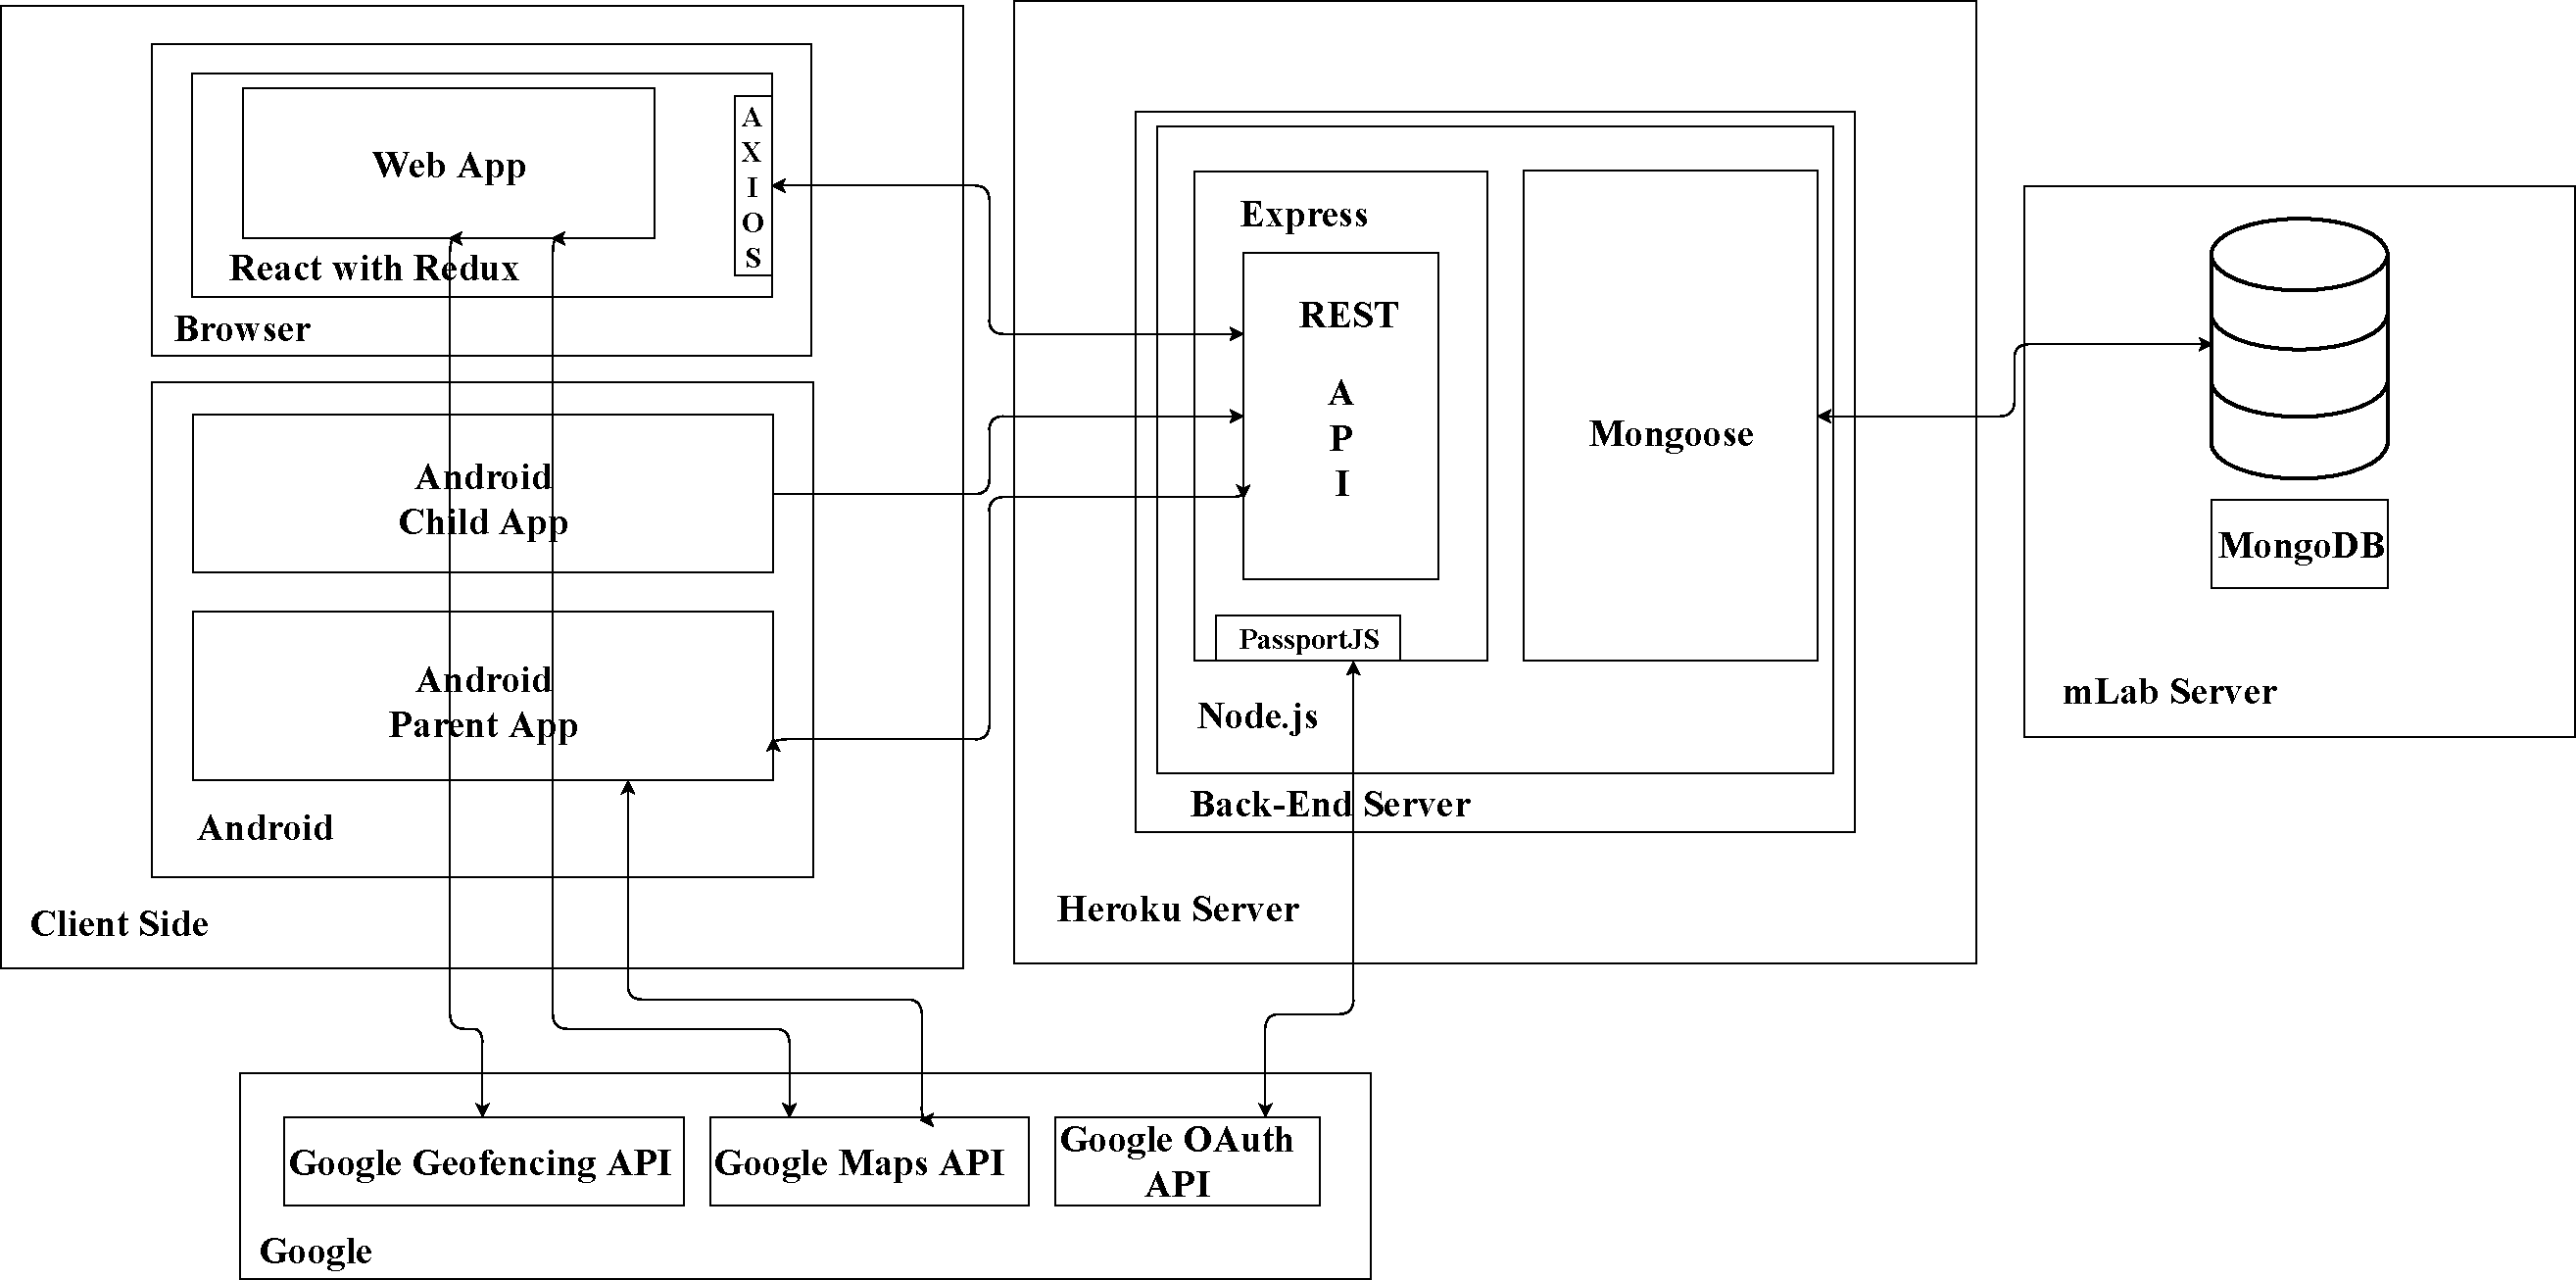
\includegraphics[width=.95\textwidth]{moduly_interfejsy_komunikacyjne}
			\end{tabular} 
			\caption{Architektura, moduły i interfejsy}
		\end{figure}

		\subsection{Frontend aplikacji webowej}

			\subsubsection{Frameworki, biblioteki i technologie}

				\begin{itemize}
					\item React - tworzenie komponentów
					\item Redux - przechowywanie i udostępnianie danych komponentom
					\item axios - tworzenie zapytań do serwera backendowego
					\item reduxThunk - umożliwia asynchroniczne oczekiwanie na odpowiedzi serwera backendowego,
					\item react-router-dom - tworzenie odnośników do różnych komponentów aplikacji
					\item react-google-maps - tworzenie komponentów React odpowiedzialnych za wyświetlanie map Google
					\item semantic-ui-react - tworzenie komponentów z stylizacją semantic ui
				\end{itemize}

			\subsubsection{Podział na foldery}

				\begin{itemize}
					\item actions - akcje wykorzystywane przez redux i reduxThunk do komunikacji frontendu z backendowym serwerem,
					\item components - komponenty React,
					\item reducers - funkcje potrzebne do prawidłowego działania redux
				\end{itemize}

			\subsubsection{Komponenty}

				\begin{itemize}
					\item App - komponent główny aplikacji zawierający BrowserRouter odpowiadający za prawidłowe wyświetlanie komponentów ze względu na ścieżke wpisaną w pole adresu przeglądarki,
					\item Header - komponent zawierający menu, wyświetlany po zalogowaniu się do aplikacji na górze ekranu,
					\item Map - komponent obsługujący wyświetlanie map Google,
					\item folder Landing - zawiera komponenty odpowiedzialne za wyświetlanie ekranu powitalnego, logowania, rejestracji i logowania za pomocą Google,
					\item folder Dashboard - zawiera komponenty wyświetlające aktualnie obowiązujące reguły i wyświetlające mapę z aktualnymi położeniami dzieci,
					\item folder Children - zwiera komponenty wyświetlające powiązane z kontem rodzica dzieci, umożliwia dodawanie nowego dziecka, edycję istniejącego i usunięcie istniejącego,
					\item folder Areas - zawiera komponenty wyświetlające powiązane z kontem rodzica obszary, umożliwia dodawanie nowego obszaru, edycję istniejącego i usunięcie istniejącego,
					\item folder Rules - zawiera komponenty wyświetlające powiązane z kontem rodzica reguły wybranego dziecka, umożliwia dodawanie nowej reguły, edycję istniejącej i usunięcie istniejącej.
				\end{itemize}
		\subsection{Backend}
		\subsubsection{Wykorzystywane pakiety Node.js}
		\begin{itemize}
			\item Express - framework używany do tworzenia serwerów w technologii Node.js
			\item concurrently - współbieżne uruchamianie skryptów
			\item mongoose - tworzenia obiektów MongoDB  
			\item nodemon - restartowanie serwera w przypadku wprowadzania zmian
			\item passport - autentyfikacja użytkowania
			\item passport-google-oauth20 - autentyfikacja przy użyciu konta google
			\item passport-local - lokalna autentyfikacja 
			\item morgan - logowanie żądań 
			\item body-parser - parsowanie żądań do serwera 
			\item bcryptjs - kryptowanie haseł
			\item cookie-session - utrzymywanie sesji i przechowywanie informacji o ciasteczkach po stronie klienta
			\item path - wspomaganie pracy ze ścieżkami plików i folderów	
		\end{itemize}
		\subsubsection{Testy i dokumentacja - Postman}
		Do testowania API użyo aplikacji postman, w której wygenerowano dokumentację, dostępną pod adresem:

		\href{https://documenter.getpostman.com/view/5735789/Rzn6v3JY}{		https://documenter.getpostman.com/view/5735789/Rzn6v3JY}.

		\subsubsection{API}

			Aplikacja komunikuje się z serwerem poprzez RESTowe API.
			
			\begin{itemize}
				\item Rodzic
				\begin{itemize}
					\item Rejestracja i logowanie
					 \begin{itemize}
						\item POST \textbackslash registration\textbackslash parent- rejestrowanie nowego rodzica,
						\item GET \textbackslash auth\textbackslash parent\textbackslash google - logowanie dziecka z Googlem,
						\item GET \textbackslash auth\textbackslash parent\textbackslash local - logowanie emailem i hasłem.		
					\end{itemize}
					\item Dzieci
					\begin{itemize}
						\item GET \textbackslash api\textbackslash parent\textbackslash children - pobranie danych o wszystkich dzieciach dla bieżącego rodzica,
						\item POST \textbackslash api\textbackslash parent\textbackslash children - tworzenie nowego dziecka,
						\item PUT \textbackslash api\textbackslash parent\textbackslash children\textbackslash :childId - modyfikacja dziecka,
						\item DELETE \textbackslash api\textbackslash parent\textbackslash children\textbackslash :childId - usuwanie dziecka.								
					\end{itemize}
					\item Reguły
					\begin{itemize}
						\item GET \textbackslash api\textbackslash parent\textbackslash rules - pobranie bieżących reguł dla wszystkich
						\item GET \textbackslash api\textbackslash parent\textbackslash rules\textbackslash :childId  - pobranie wszystkich reguł dla określonego dziecka
						\item POST \textbackslash api\textbackslash parent\textbackslash rules - dodanie nowej reguły 
						\item PUT \textbackslash api\textbackslash parent\textbackslash rules\textbackslash :ruleId - modyfikacja wybranej reguły,
						\item DELETE \textbackslash api\textbackslash parent\textbackslash rules\textbackslash :ruleId - usuwanie wybranej reguły.		
					\end{itemize}
					\item Obszary
					\begin{itemize}		
						\item GET \textbackslash api\textbackslash parent\textbackslash areas - pobranie wszystkich obaszarów dla bieżącego użytkownia,
						\item POST \textbackslash api\textbackslash parent\textbackslash areas - tworzenie nowego obszaru,
						\item PUT \textbackslash api\textbackslash parent\textbackslash areas\textbackslash :areaId - modyfikacja wybranego obszaru,
						\item DELETE \textbackslash api\textbackslash parent\textbackslash  areas\textbackslash :areaId - usuwanie wybranego obszaru.	
					\end{itemize}
					\item Lokalizacja
					\begin{itemize}
						\item GET \textbackslash api\textbackslash parent\textbackslash location\textbackslash :childId - pobranie loklizacja wybranego dziecka
					\end{itemize}
					\item Łącznie z dzieckiem
					\begin{itemize}
						\item GET \textbackslash api\textbackslash parent\textbackslash code\textbackslash :codeValue - pobranie dziecka o podanym kodzie
					\end{itemize}
				\end{itemize}
				\item Dziecko
				\begin{itemize}
					\item Rejestracja i logowanie
					\begin{itemize}
						\item POST \textbackslash registration \textbackslash child
						\item GET \textbackslash auth\textbackslash child\textbackslash google - logowanie dziecka z Googlem,
						\item GET \textbackslash auth\textbackslash child\textbackslash local - logowanie dziecka emailem i hasłem,	
					\end{itemize}
					\item Lokalizacja
					\begin{itemize}
						\item POST \textbackslash api\textbackslash child\textbackslash location - dodaje lokalizacje do dziecka i aktualizuje czas jej dodania
						\item GET \textbackslash api\textbackslash child\textbackslash location - pobranie lokalizacji ostatniej lokalizacji dziecka z bazy danych		
					\end{itemize}				
						\item Łączenie z rodziciem
					\begin{itemize}
						\item GET \textbackslash api\textbackslash child\textbackslash code - pobranie nowo utworzonego kodu łączenia						
					\end{itemize}

				\end{itemize}
				\item Użytkownik
				\begin{itemize}
					\item \textbackslash api\textbackslash current\_user - zwraca bieżącego zalogowanego użytkownika,
					\item \textbackslash api\textbackslash logout - wylogowanie użytkownika.
				\end{itemize}
			\end{itemize}
		
		\subsection{Diagramy bazy danych}

			\begin{figure}[H] 
				\centering
				\begin{tabular}{c}
					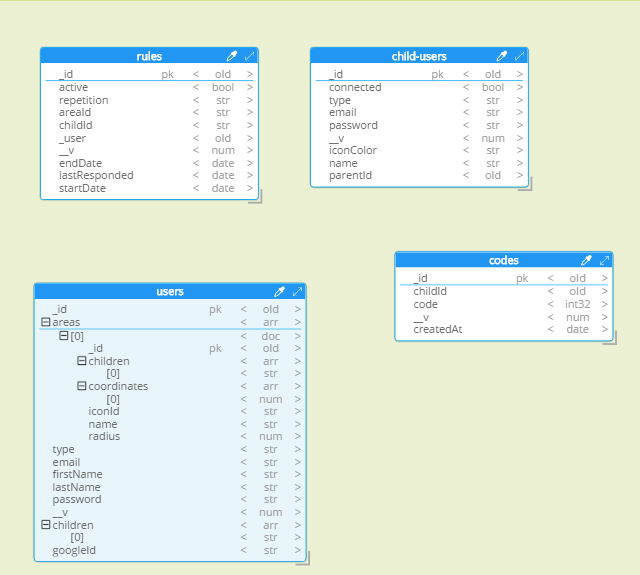
\includegraphics[width=.95\textwidth]{relacjeWBazie.png}
				\end{tabular} 
				\caption{Dokumenty w bazie danych}
			\end{figure}

			\begin{figure}[H] 
				\centering 
				\begin{tabular}{c}
					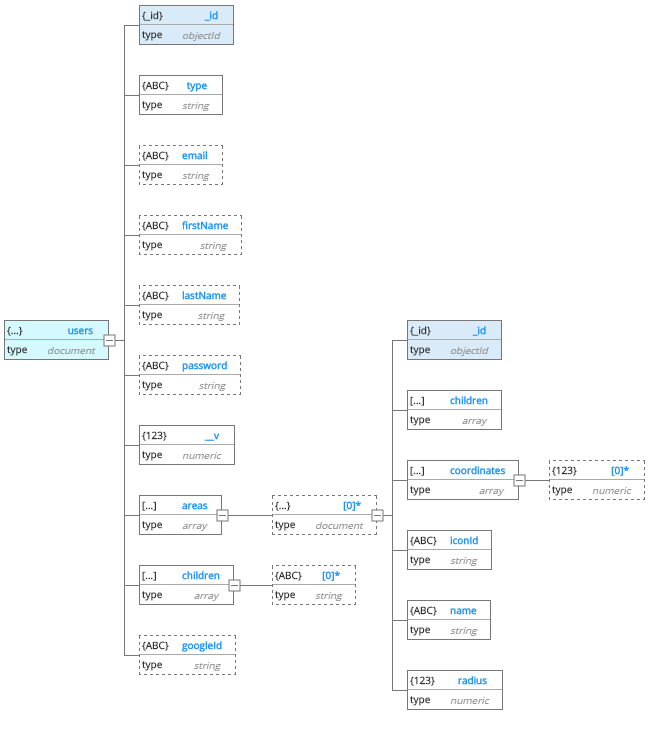
\includegraphics[]{users.png} 
				\end{tabular} 
				\caption{Schemat dokumentu użytkownika rodzica}
			\end{figure}

			\begin{figure}[H] 
				\centering 
				\begin{tabular}{c}
					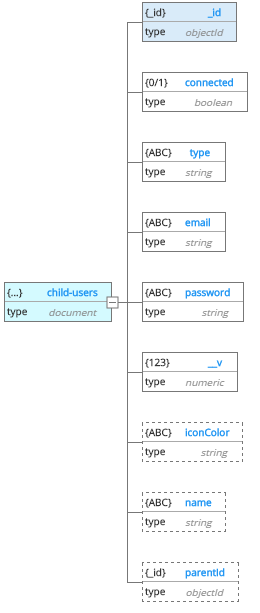
\includegraphics[]{childUser.png} 
				\end{tabular} 
				\caption{Schemat dokumentu użytkownika dziecka}
			\end{figure}

			\begin{figure}[H] 
				\centering 
				\begin{tabular}{c}
					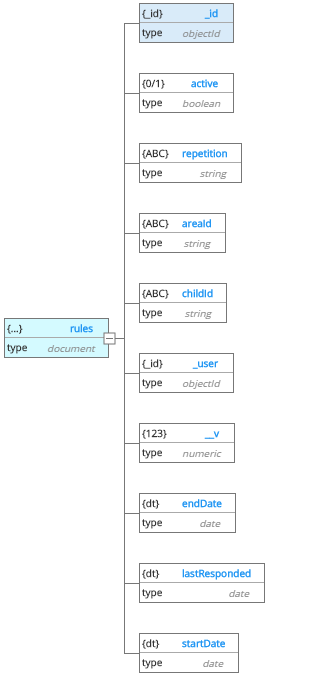
\includegraphics[]{rules.png} 
				\end{tabular} 
				\caption{Schemat dokumentu relacji}
			\end{figure}

			\begin{figure}[H] 
				\centering 
				\begin{tabular}{c}
					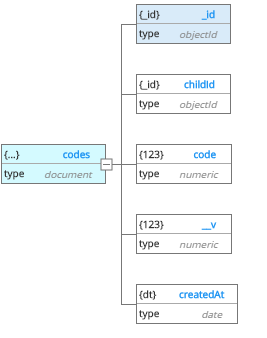
\includegraphics[]{codes.png} 
				\end{tabular} 
				\caption{Schemat dokumentu kodu}
			\end{figure}



	\section{Testy automatyczne (jednostkowe i funkcjonalne) aplikacji}

	\begin{figure}[H]
    		\centering
    		\begin{tabular}{c}
    			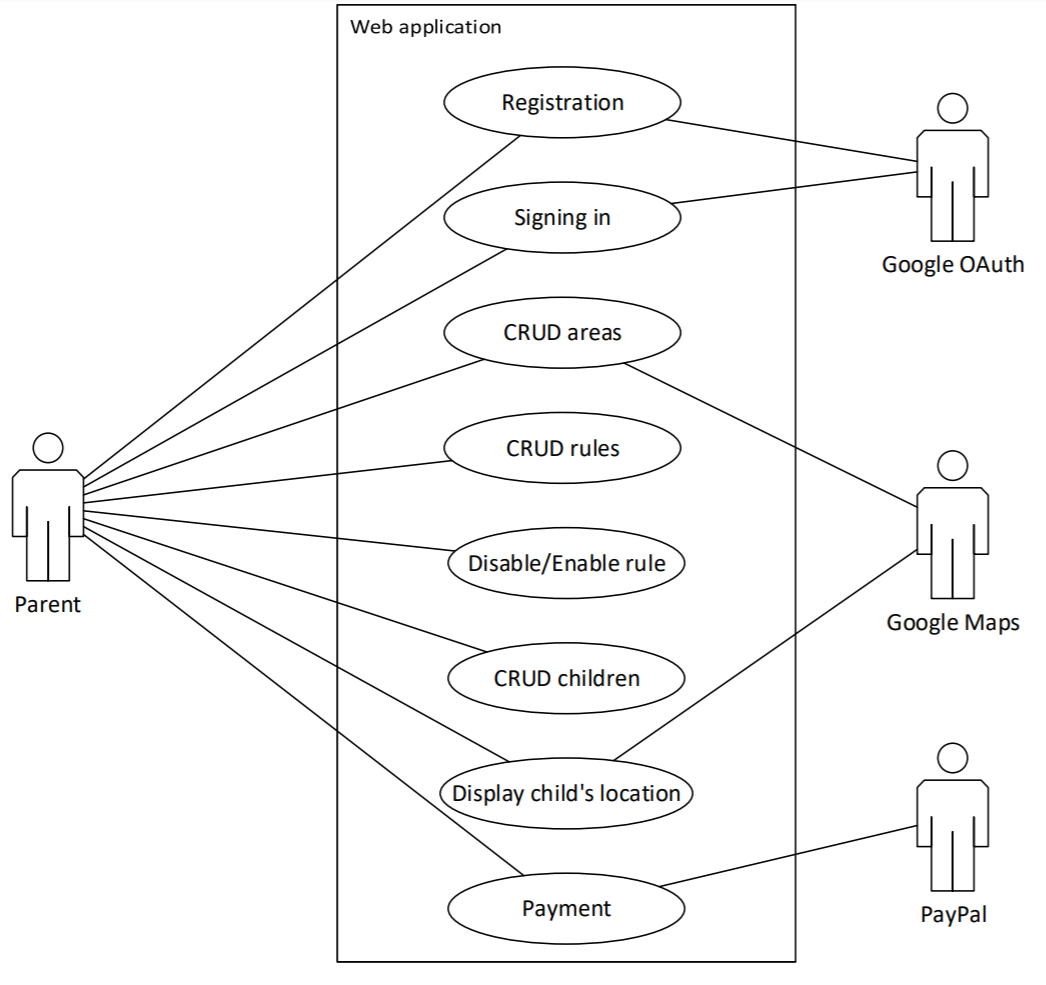
\includegraphics[width=.80\textwidth]{webUseCase}
    		\end{tabular}
    		\caption{Use cases for web application}
    	\end{figure}

    	\begin{figure}[H]
    		\centering
    		\begin{tabular}{c}
    			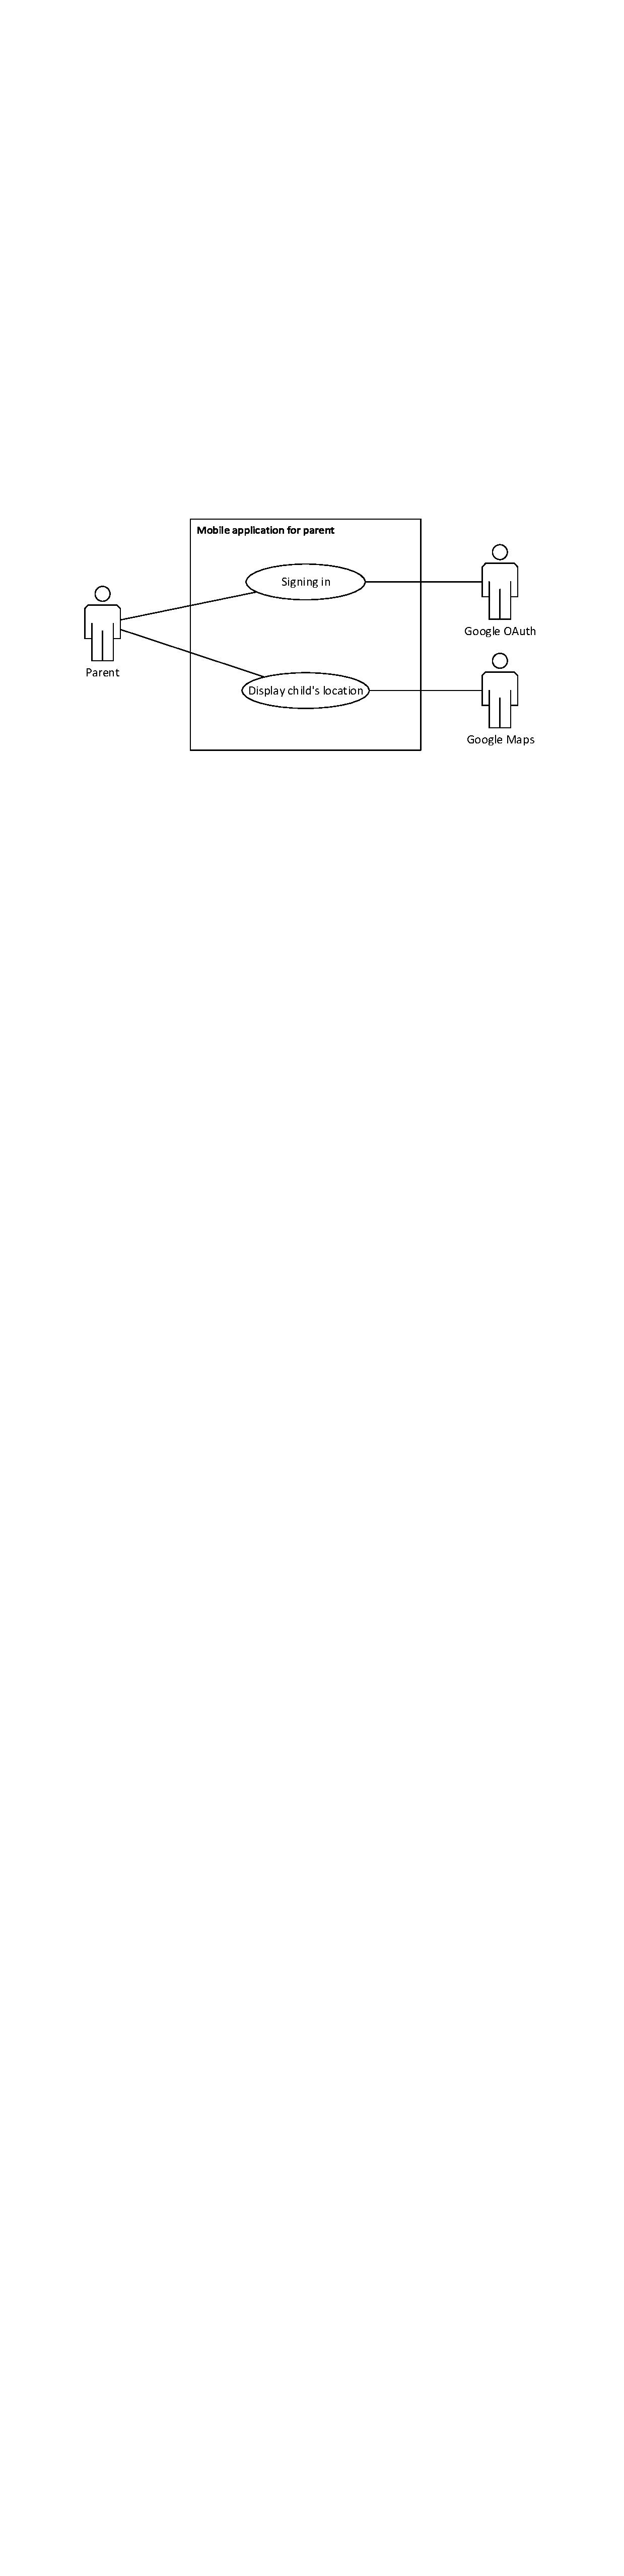
\includegraphics[width=.80\textwidth]{parentUseCase}
    		\end{tabular}
    		\caption{Use cases for parent's mobile application}
    	\end{figure}

    	\begin{figure}[H]
    		\centering
    		\begin{tabular}{c}
    			
\includegraphics[width=.80\textwidth]{childUseCase}
    		\end{tabular}
    		\caption{Use cases for child's mobile application}
    	\end{figure}

    	\begin{figure}[H]
    		\centering
    		\begin{tabular}{c}
    			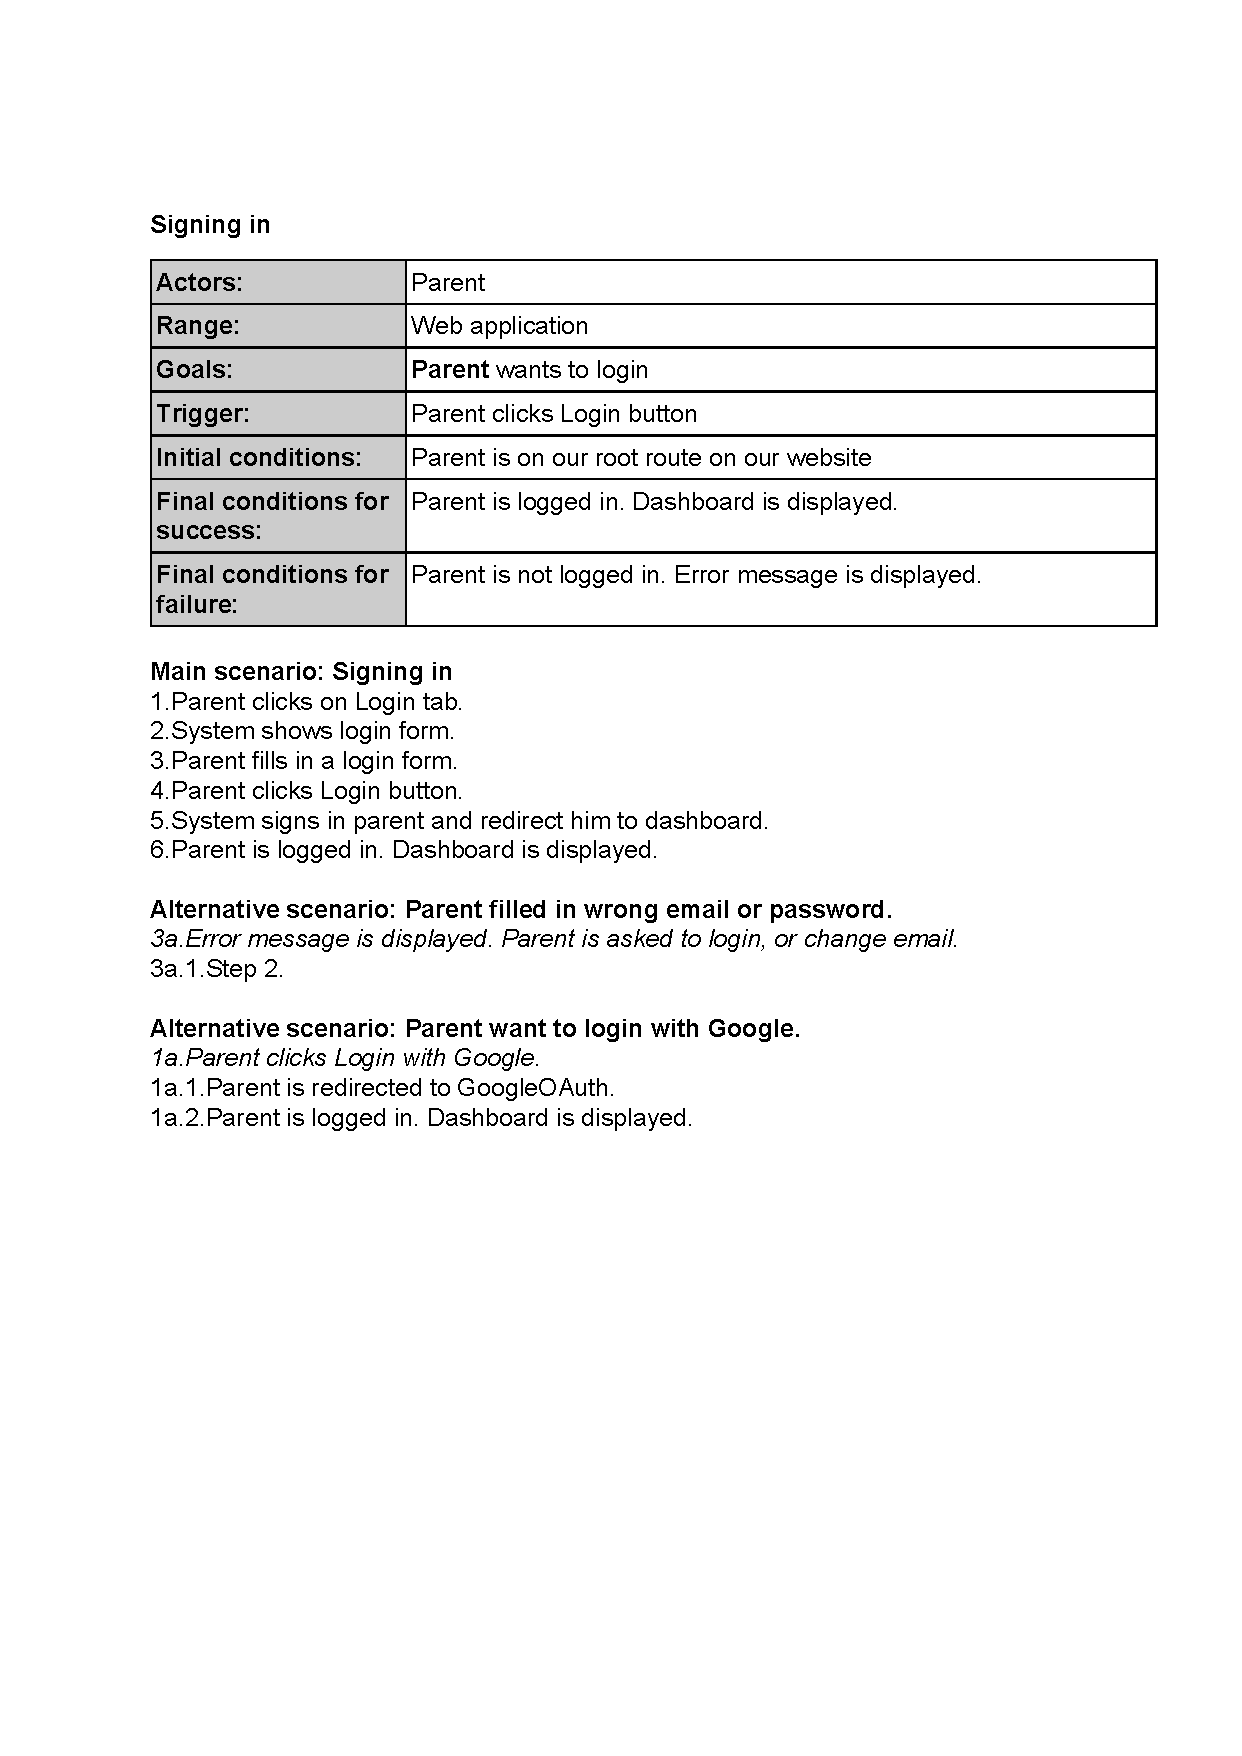
\includegraphics[width=.80\textwidth]{log_cropped}
    		\end{tabular}
    		\caption{Signing in scenario}
    	\end{figure}

    	\begin{figure}[H]
    		\centering
    		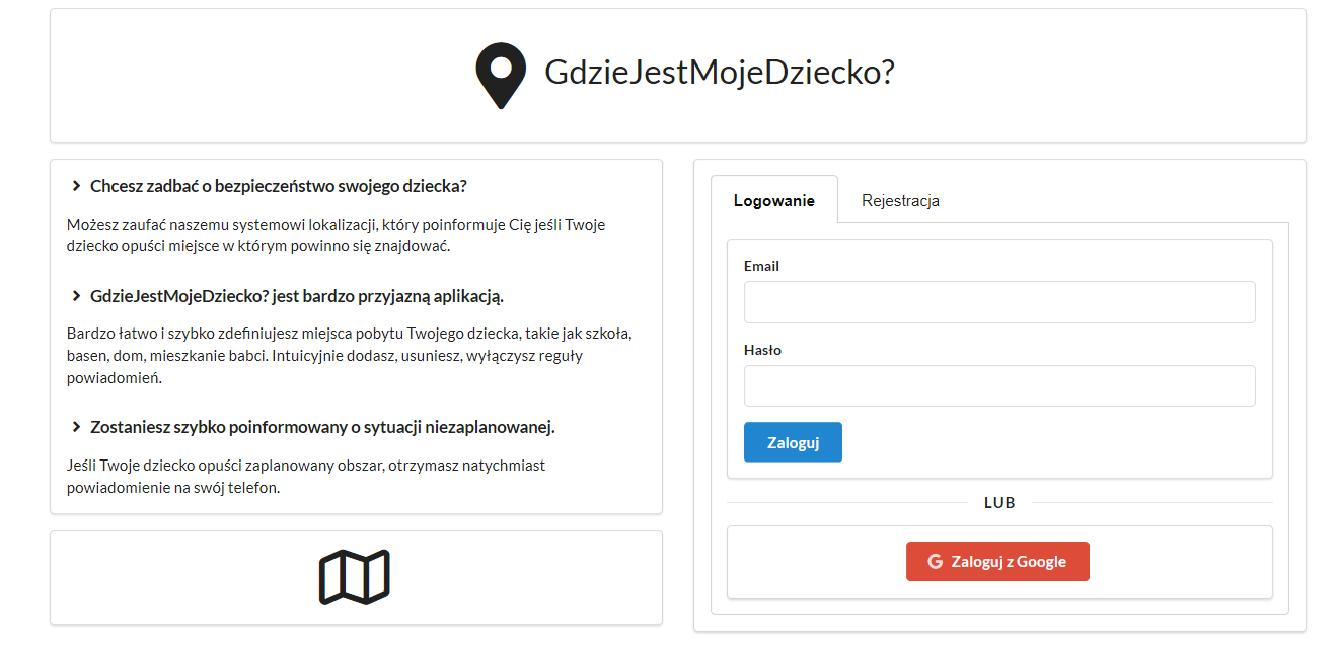
\includegraphics[width=.80\textwidth]{signinIn}
    		\caption{Signing in}
    	\end{figure}

    	\begin{figure}[H]
    		\centering
    		\begin{tabular}{c}
    			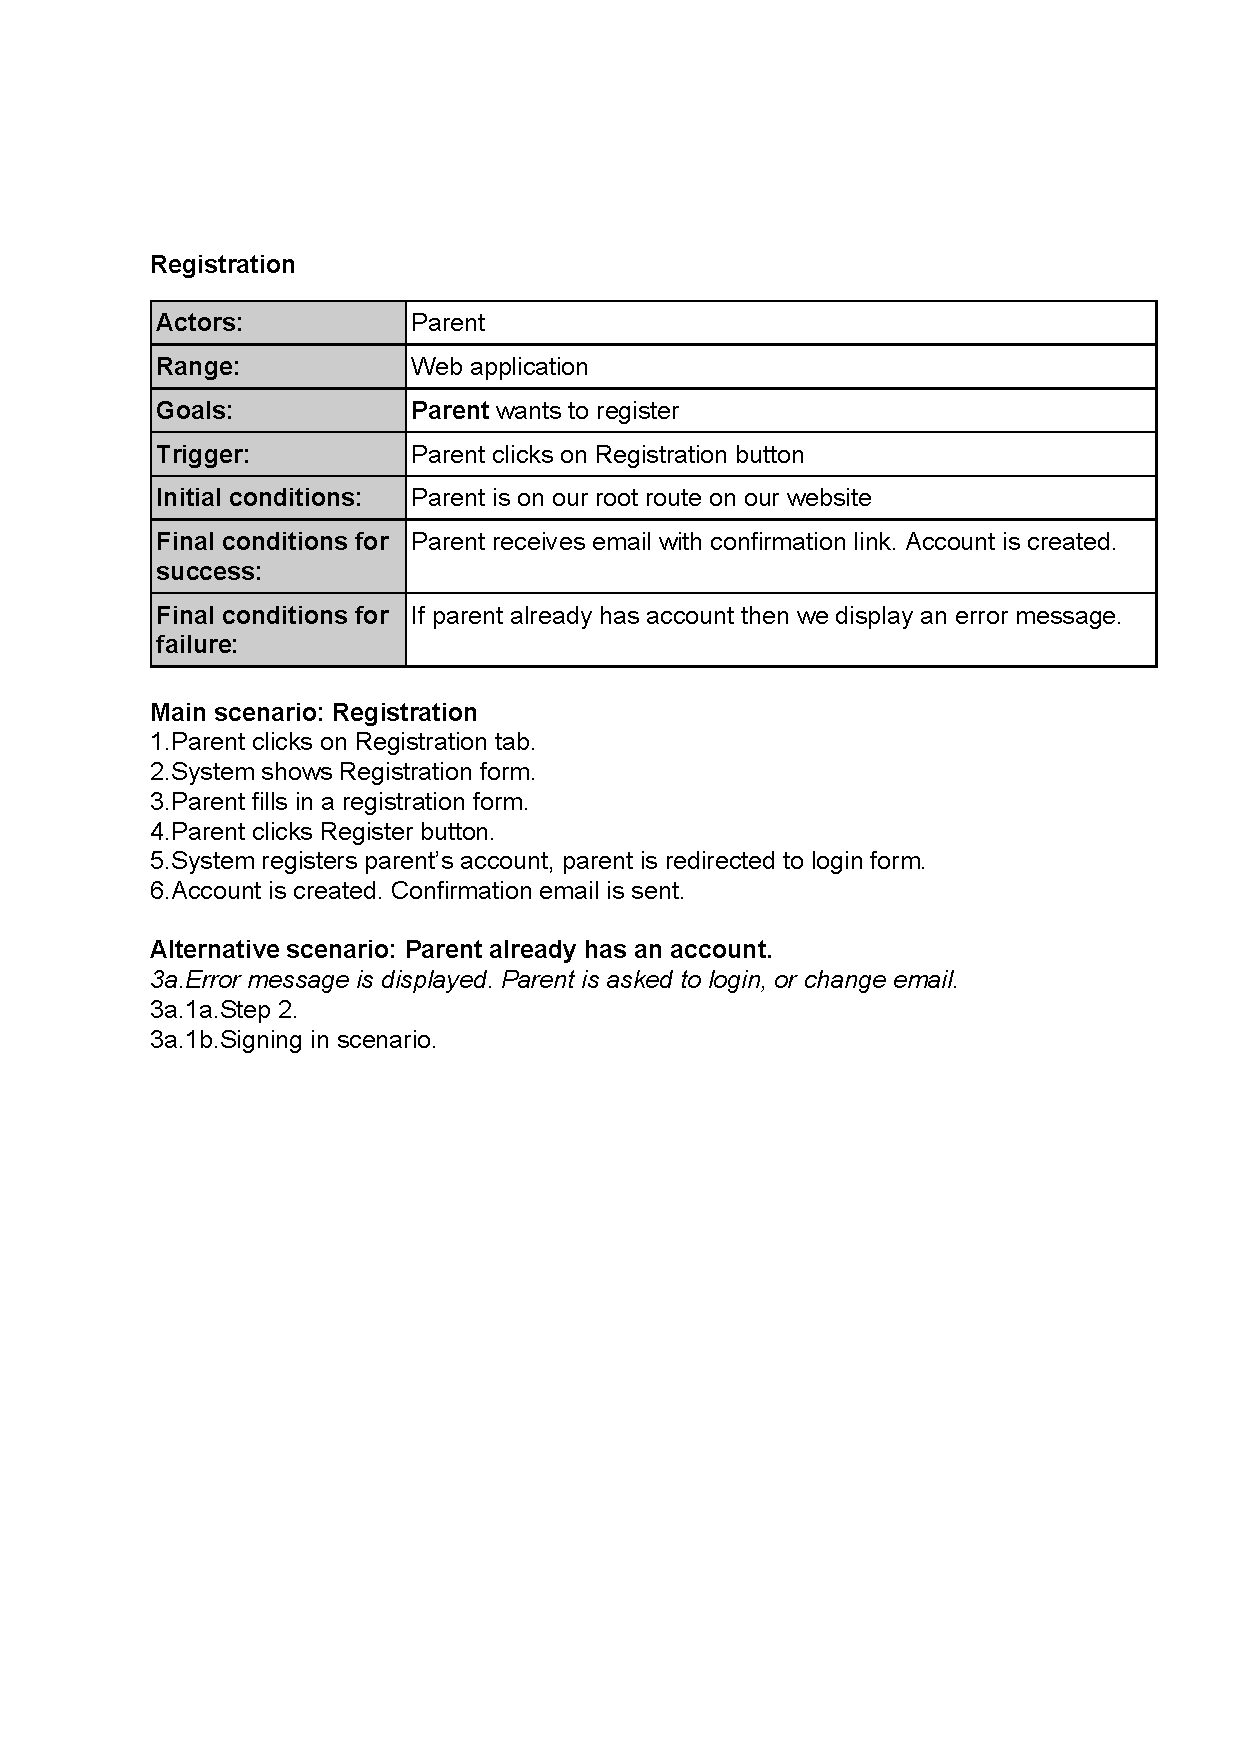
\includegraphics[width=.80\textwidth]{reg_cropped}
    		\end{tabular}
    		\caption{Registration scenario}
    	\end{figure}

    	\begin{figure}[H]
    		\centering
    		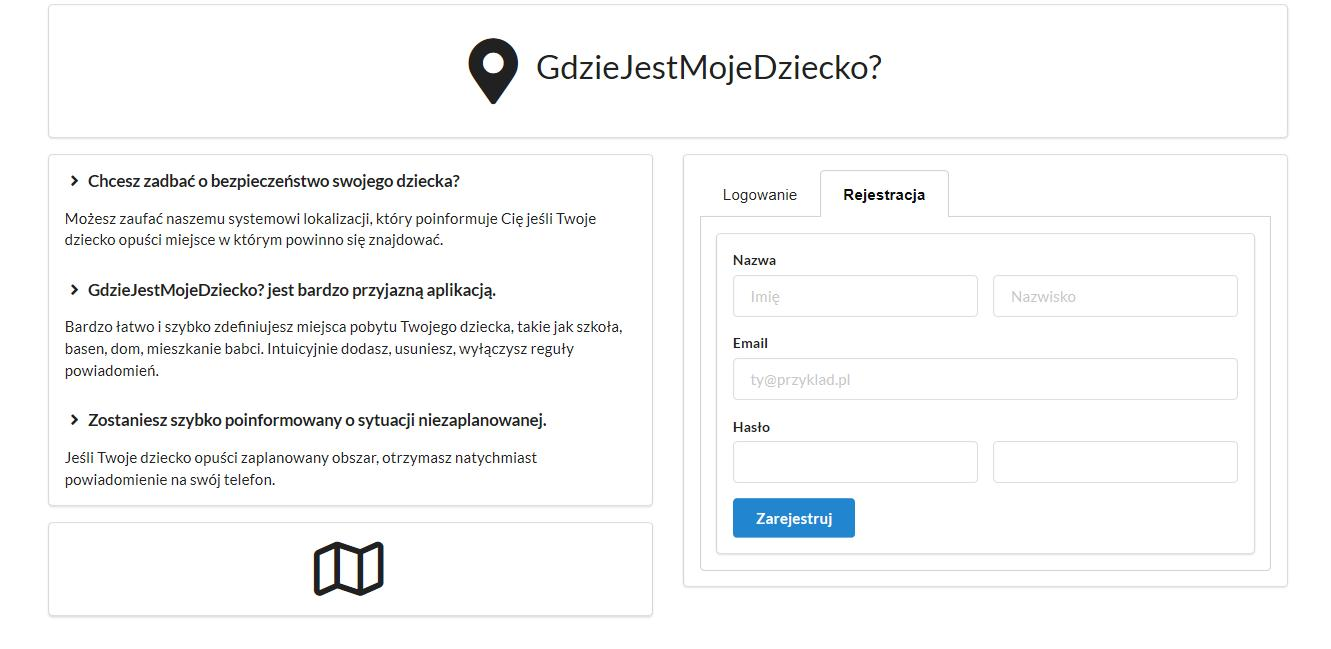
\includegraphics[width=.80\textwidth]{register}
    		\caption{Registering}
    	\end{figure}

    	\begin{figure}[H]
    		\centering
    		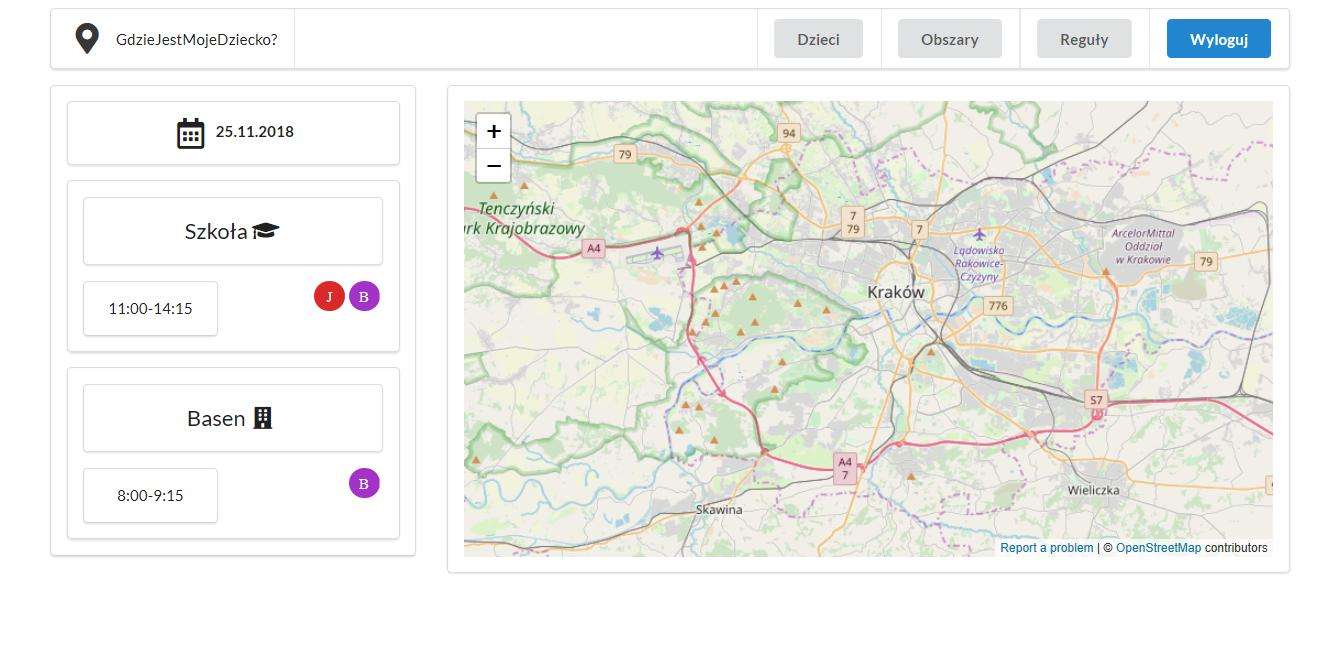
\includegraphics[width=.80\textwidth]{dashboard}
    		\caption{Dashboard}
    	\end{figure}

    	\begin{figure}[H]
    		\centering
    		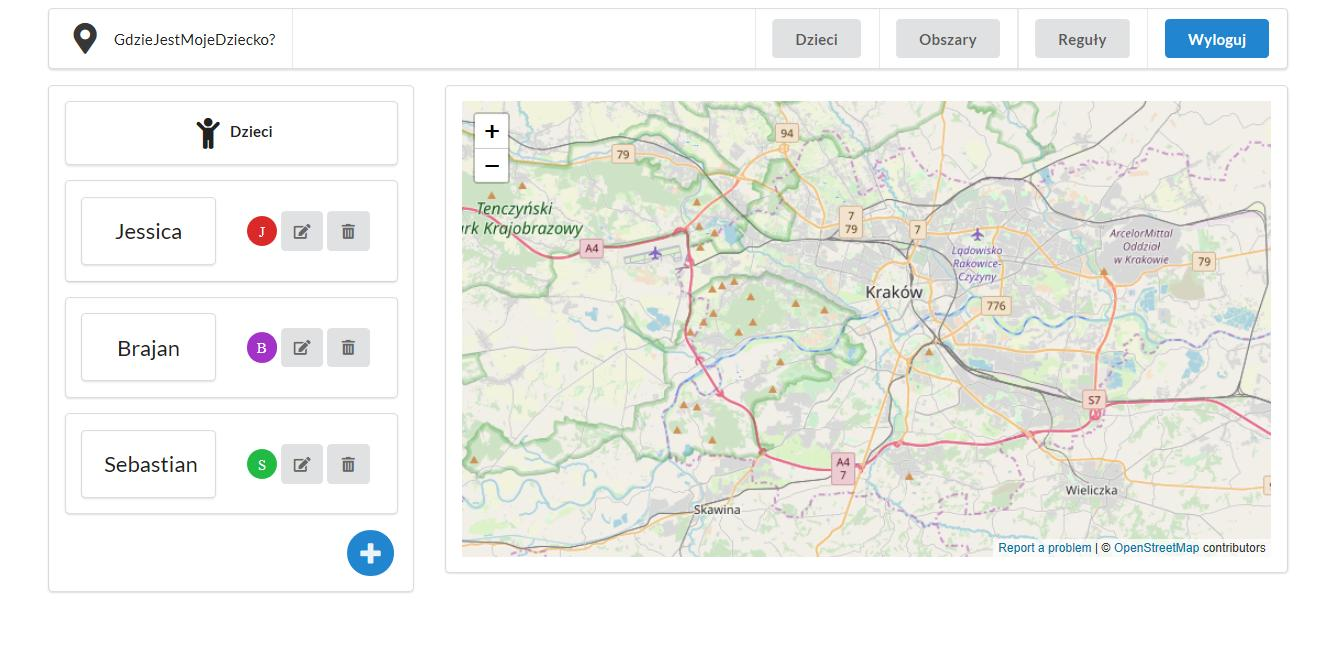
\includegraphics[width=.80\textwidth]{children}
    		\caption{Children}
    	\end{figure}

    	\begin{figure}[H]
    		\centering
    		\begin{tabular}{c}
    			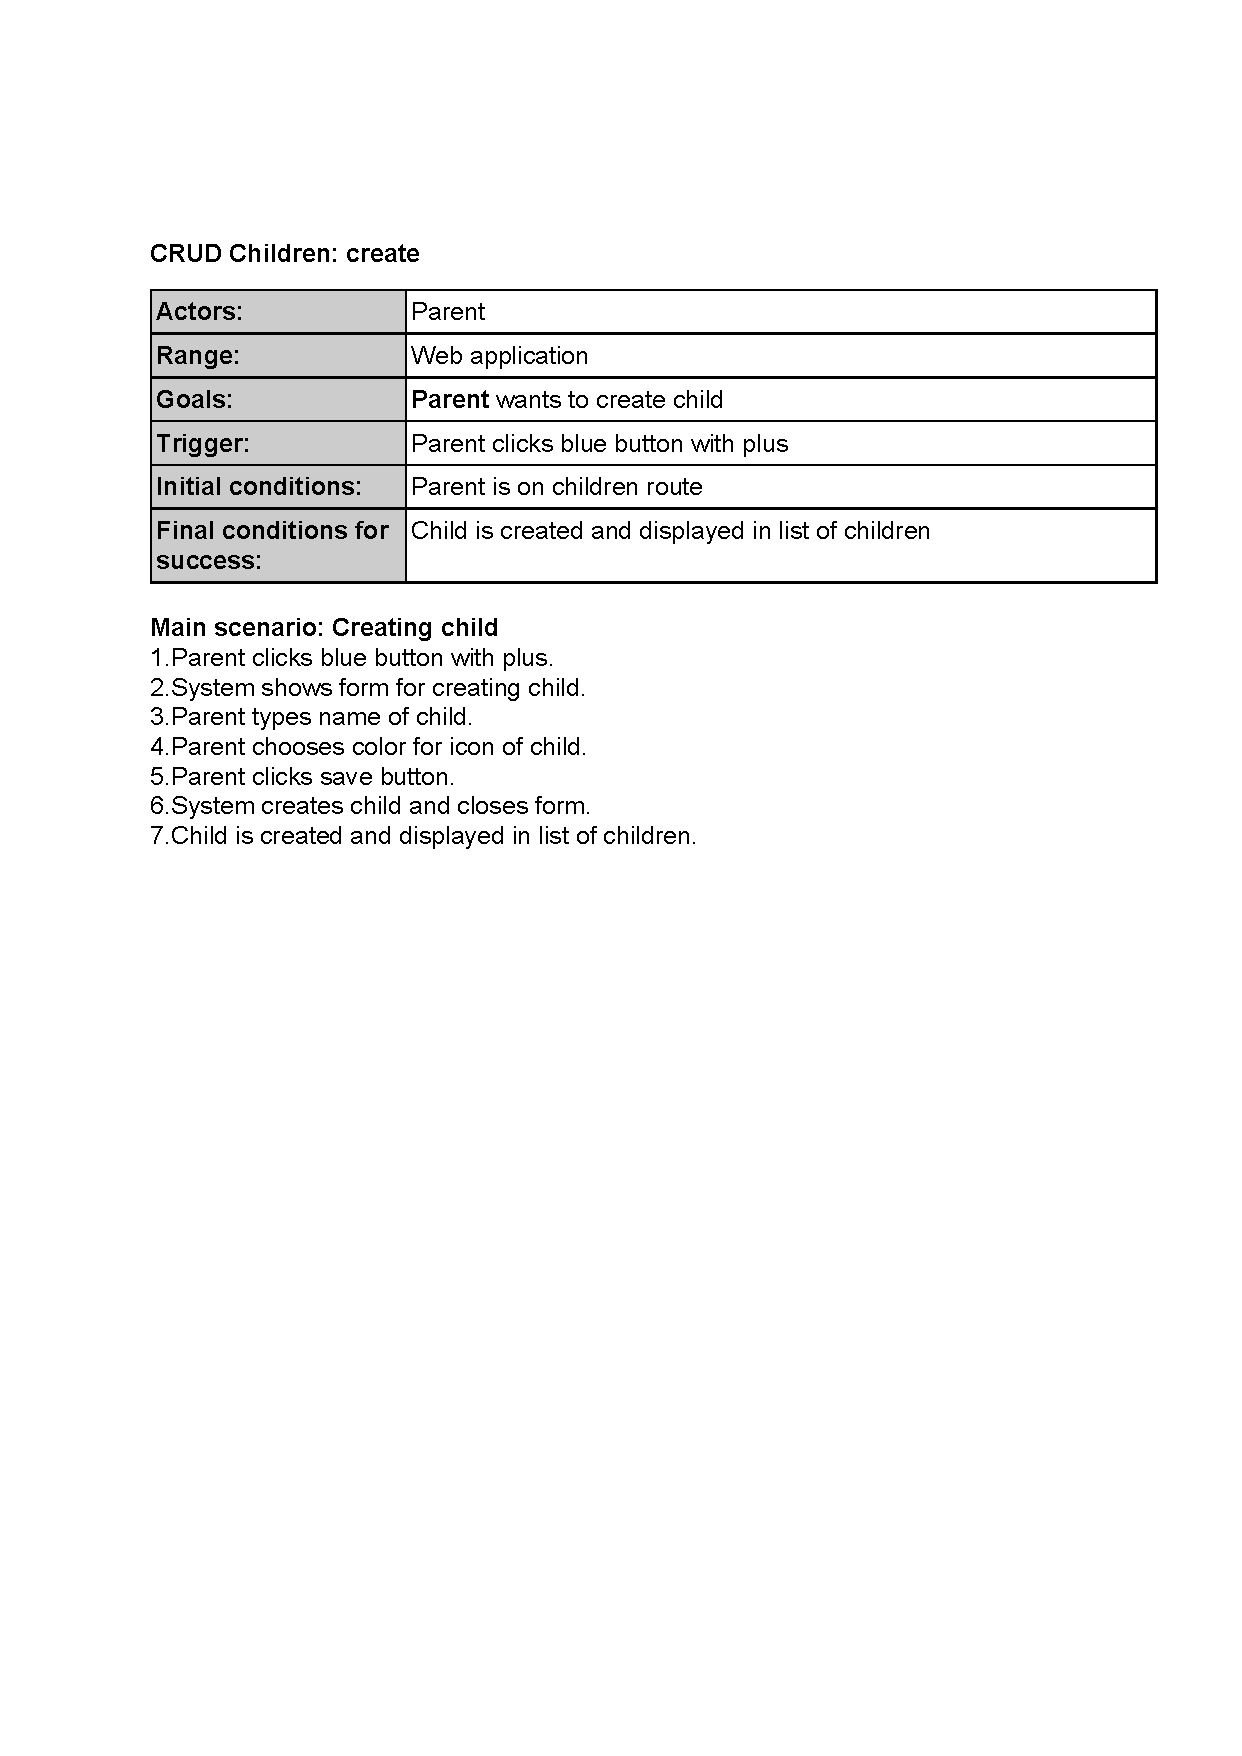
\includegraphics[width=.80\textwidth]{crC_cropped}
    		\end{tabular}
    		\caption{Creating child scenario}
    	\end{figure}

    	\begin{figure}[H]
    		\centering
    		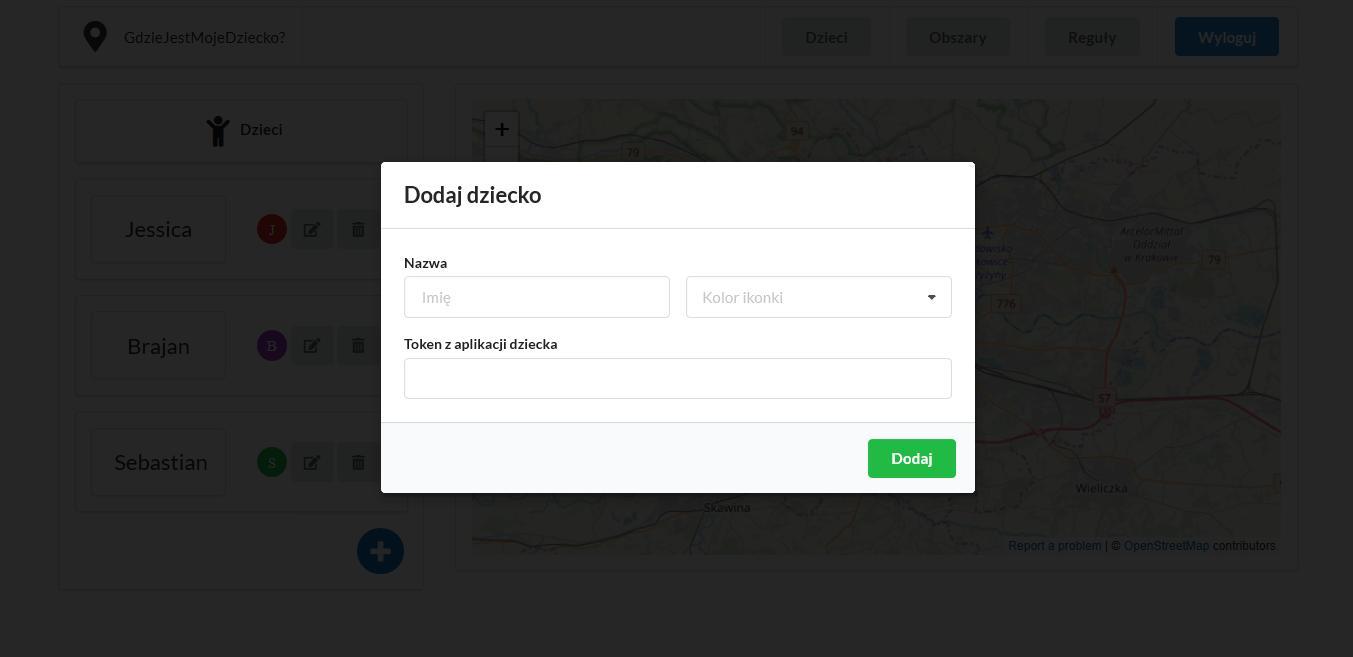
\includegraphics[width=.80\textwidth]{addChild}
    		\caption{Creating child}
    	\end{figure}

    	\begin{figure}[H]
    		\centering
    		\begin{tabular}{c}
    			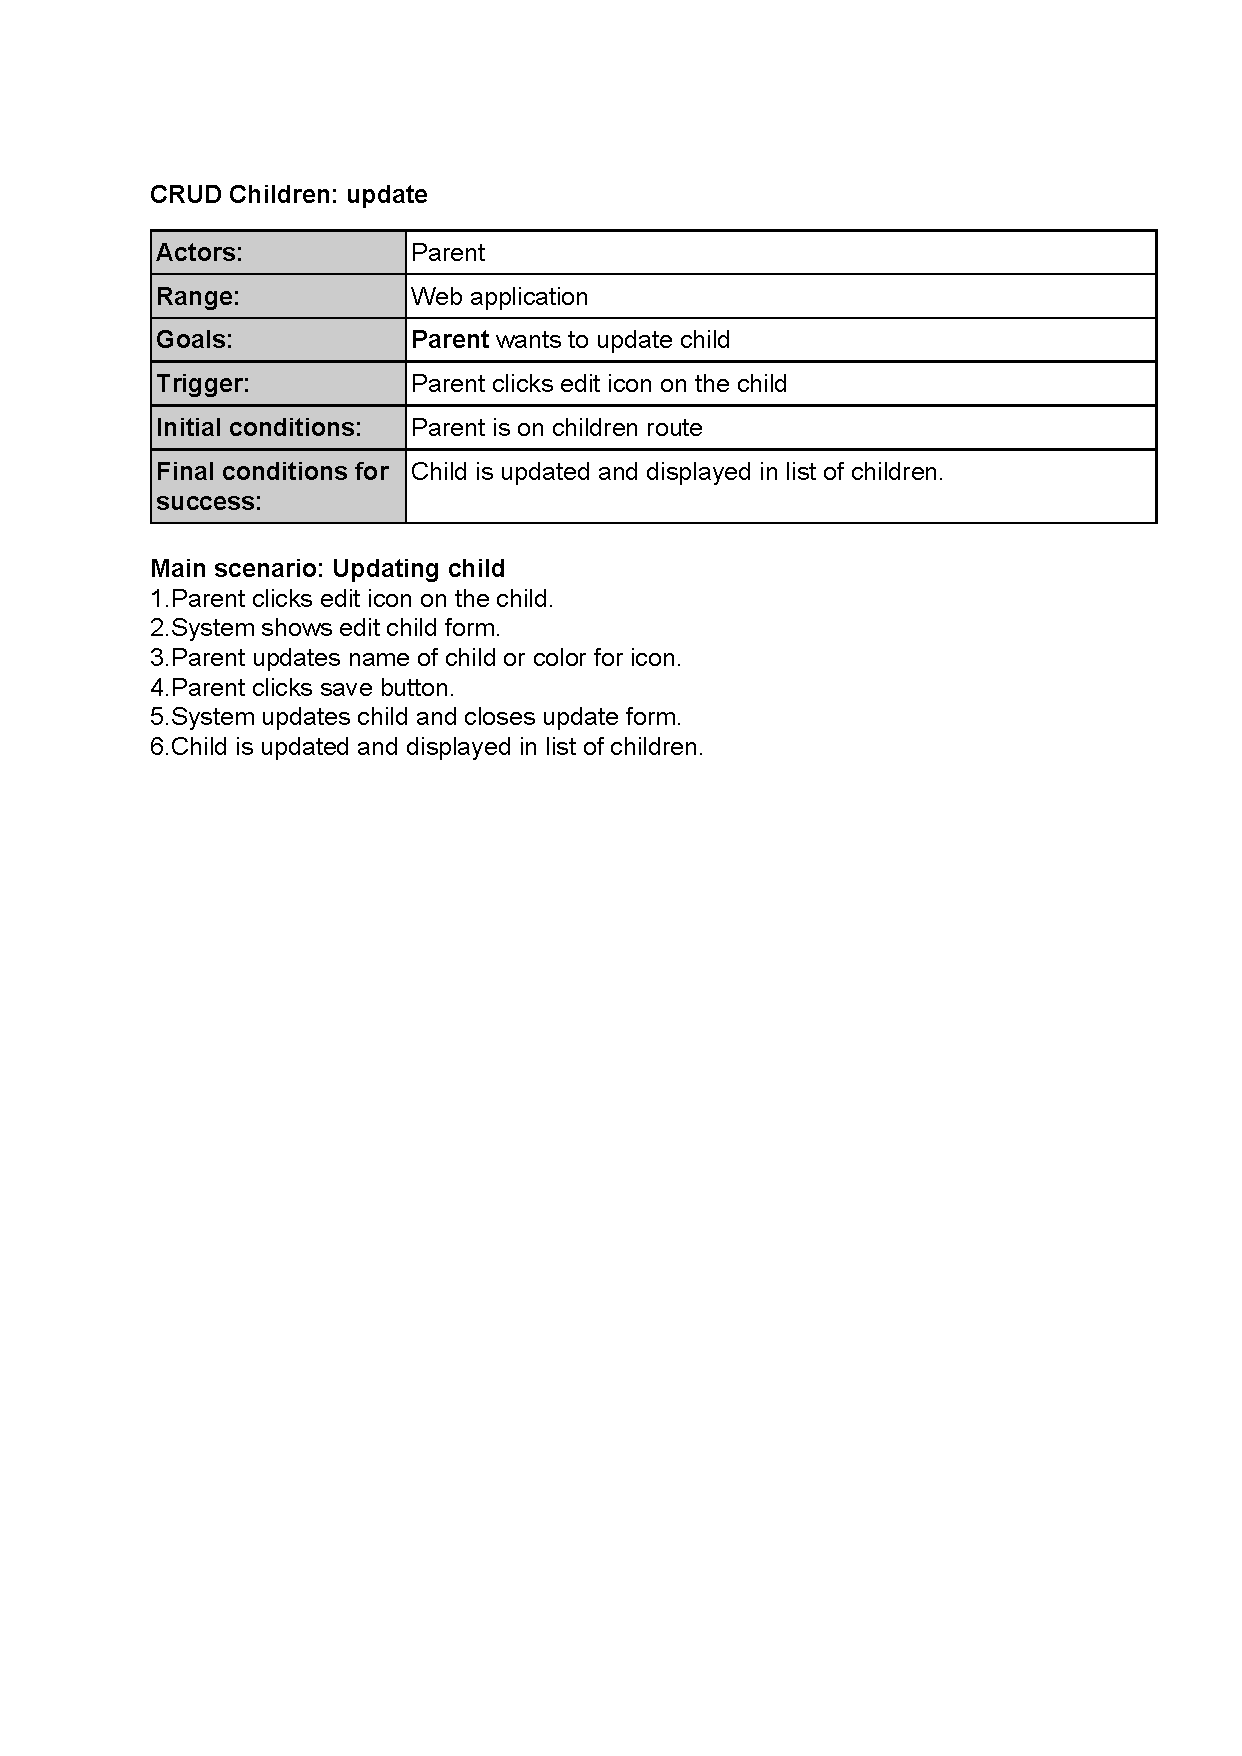
\includegraphics[width=.80\textwidth]{upC_cropped}
    		\end{tabular}
    		\caption{Updating child scenario}
    	\end{figure}

    	\begin{figure}[H]
    		\centering
    		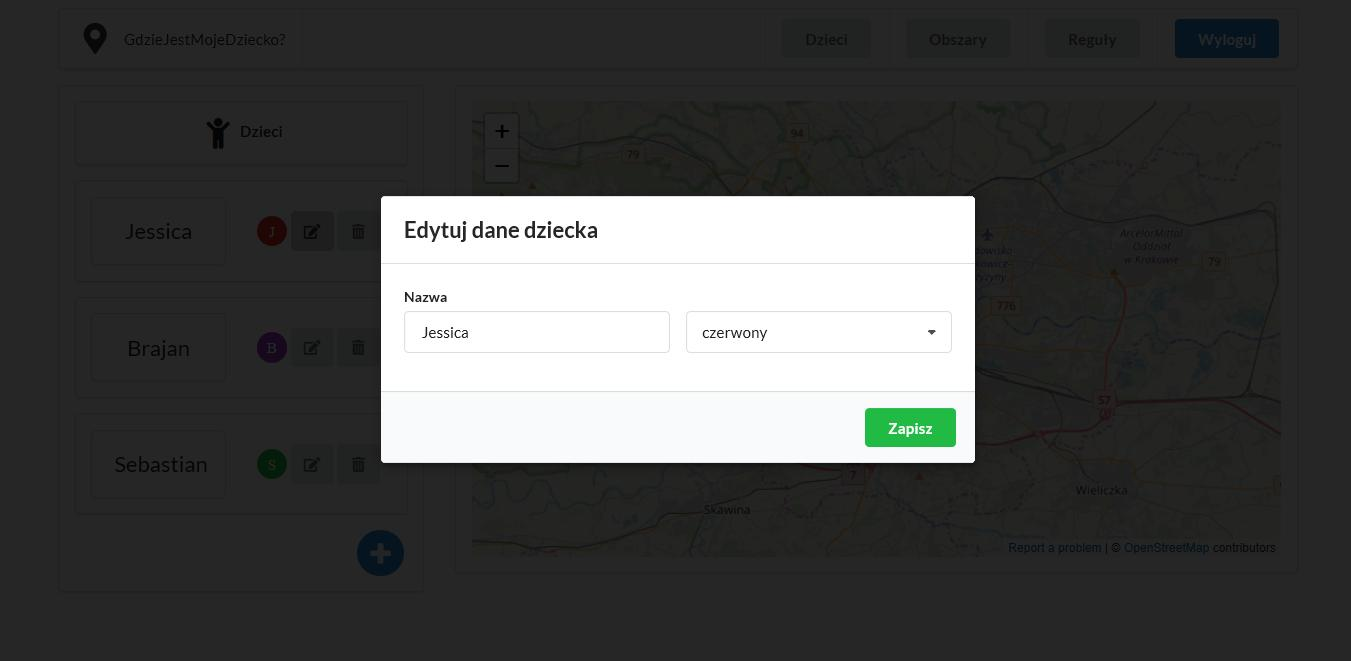
\includegraphics[width=.80\textwidth]{editChild}
    		\caption{Editing child data}
    	\end{figure}

    	\begin{figure}[H]
    		\centering
    		\begin{tabular}{c}
    			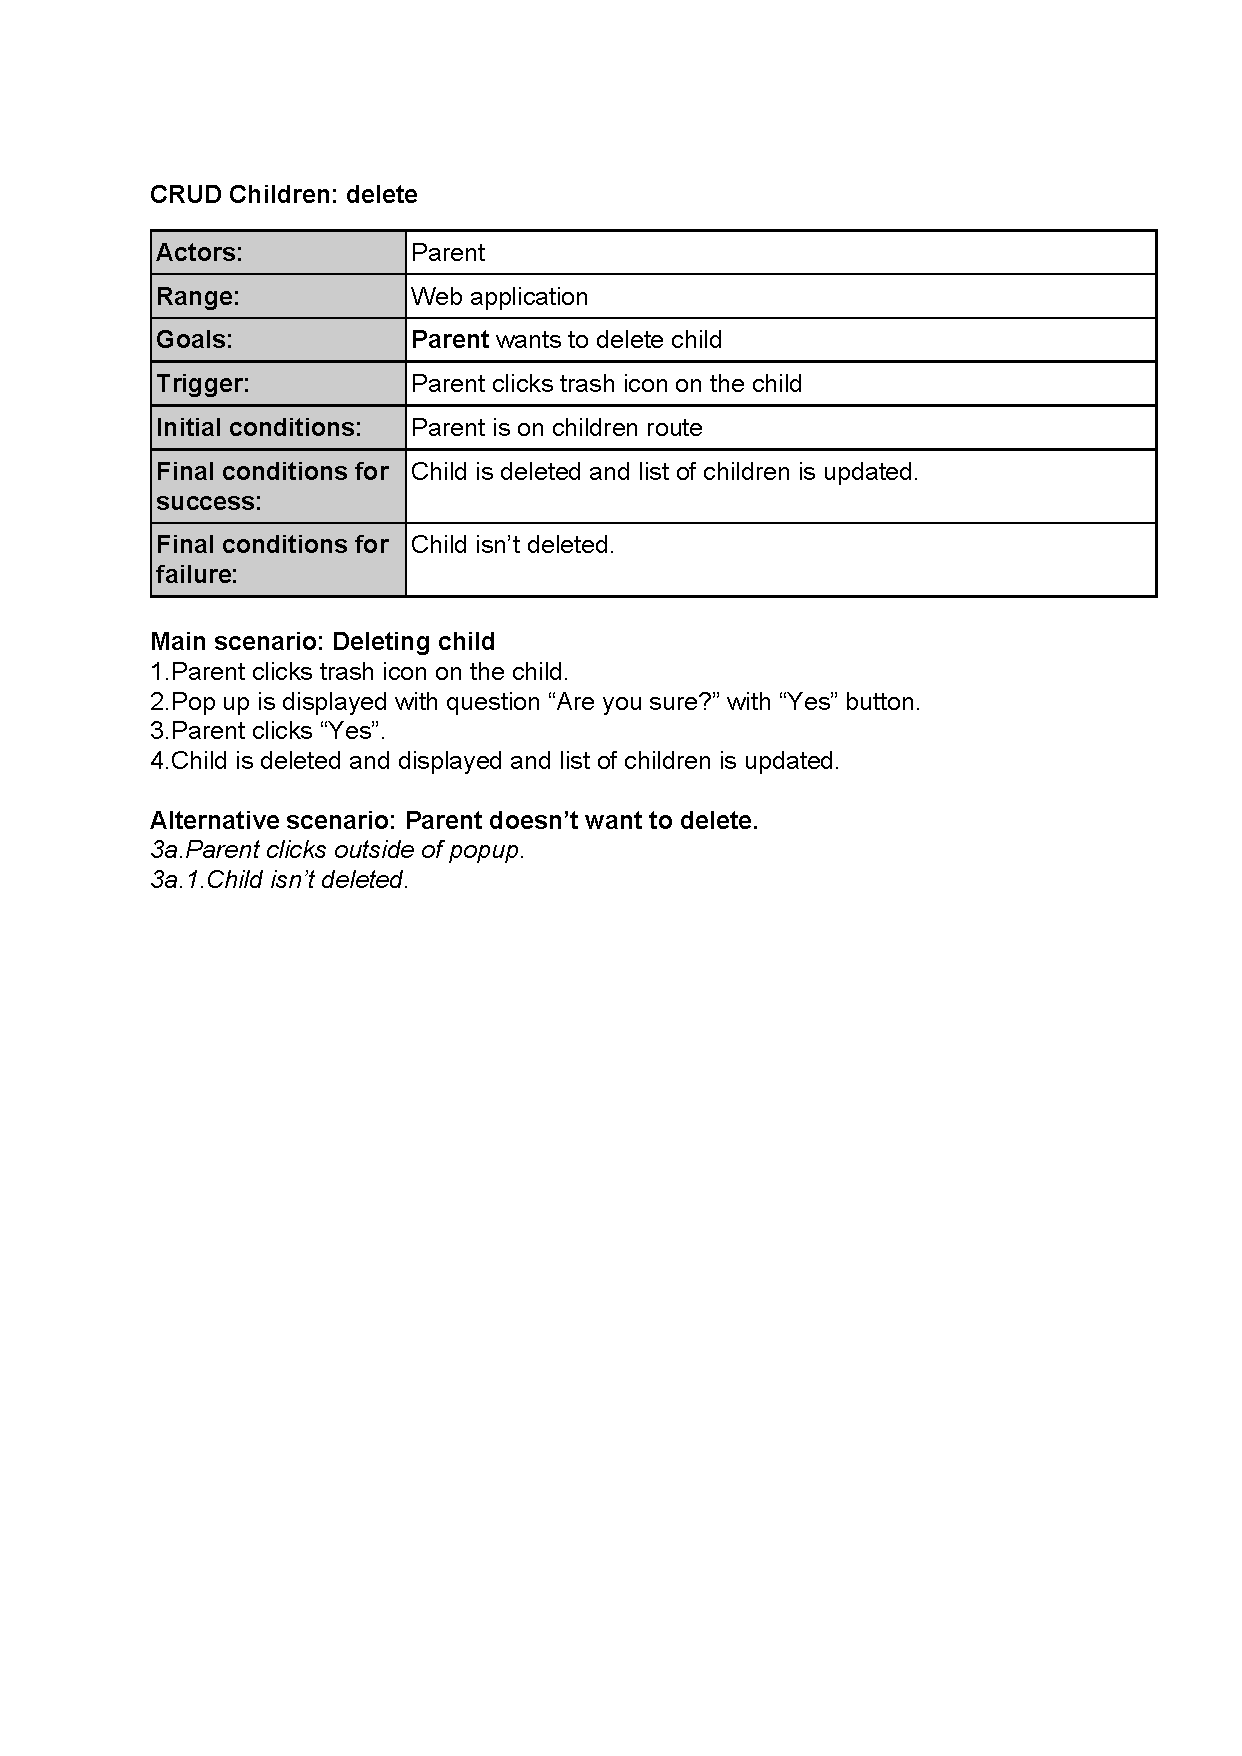
\includegraphics[width=.80\textwidth]{deC_cropped}
    		\end{tabular}
    		\caption{Deleting child scenario}
    	\end{figure}

    	\begin{figure}[H]
    		\centering
    		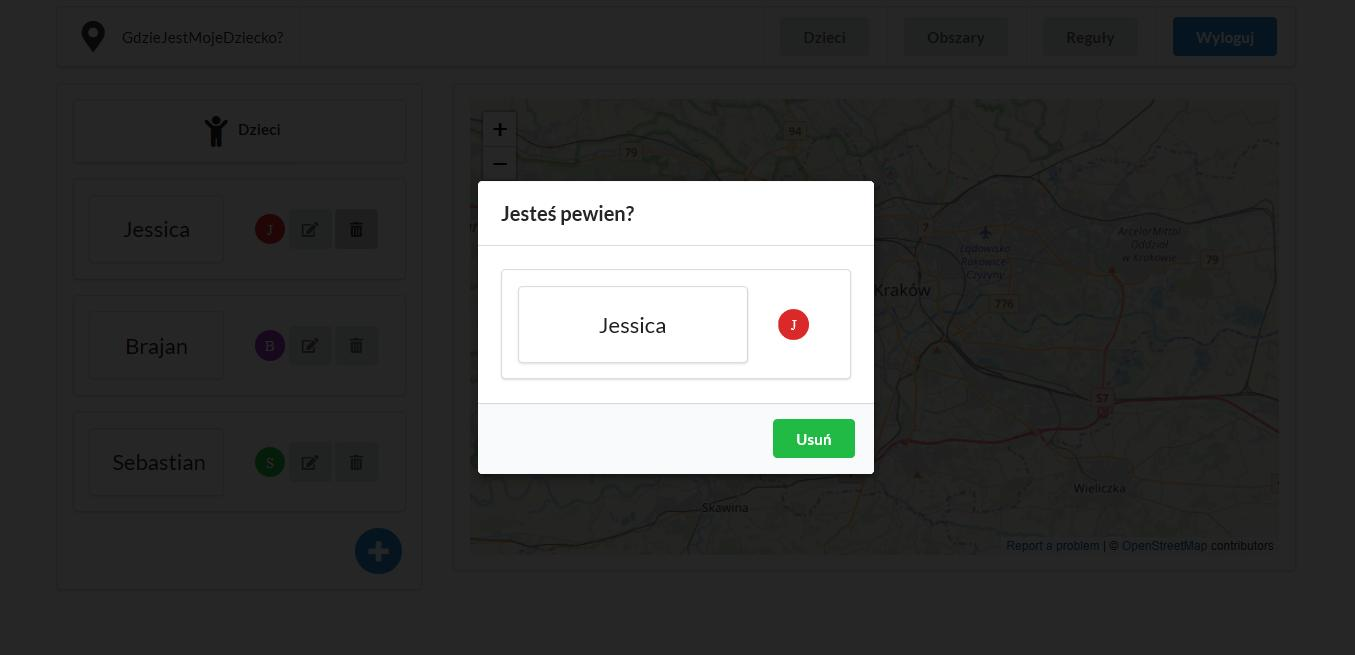
\includegraphics[width=.80\textwidth]{deleteChild}
    		\caption{Deleting child}
    	\end{figure}

    	\begin{figure}[H]
    		\centering
    		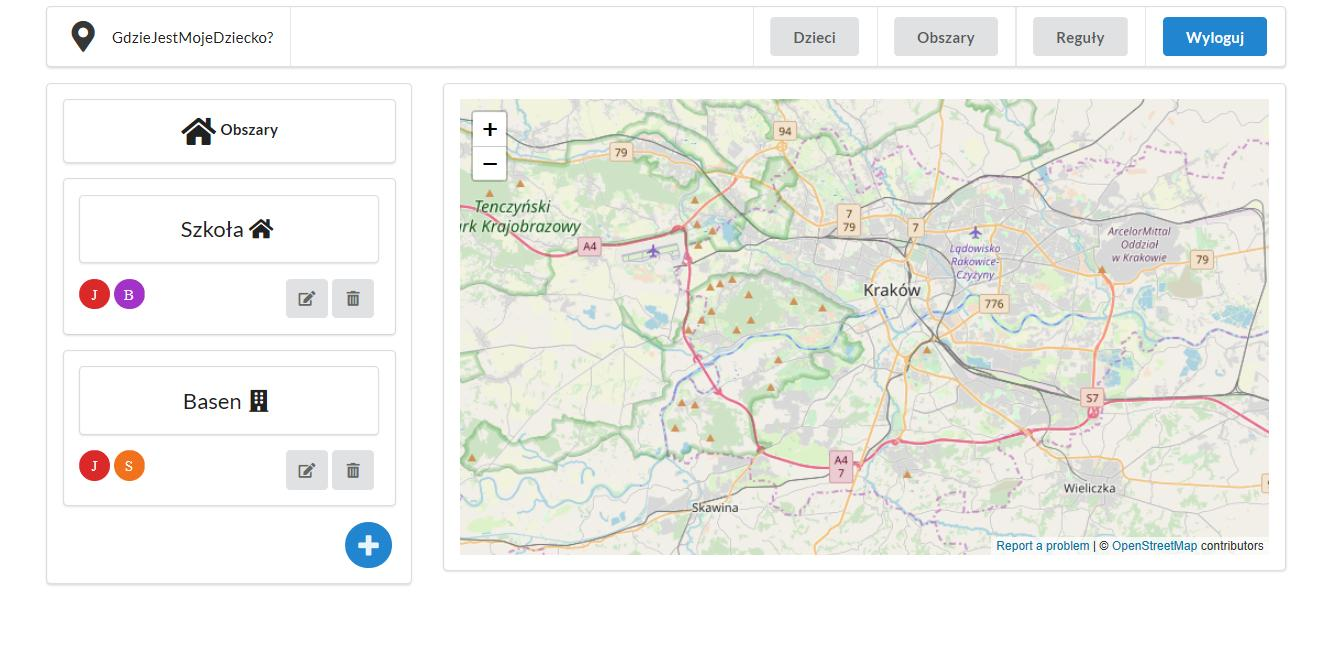
\includegraphics[width=.80\textwidth]{areas}
    		\caption{Areas}
    	\end{figure}

    	\begin{figure}[H]
    		\centering
    		\begin{tabular}{c}
    			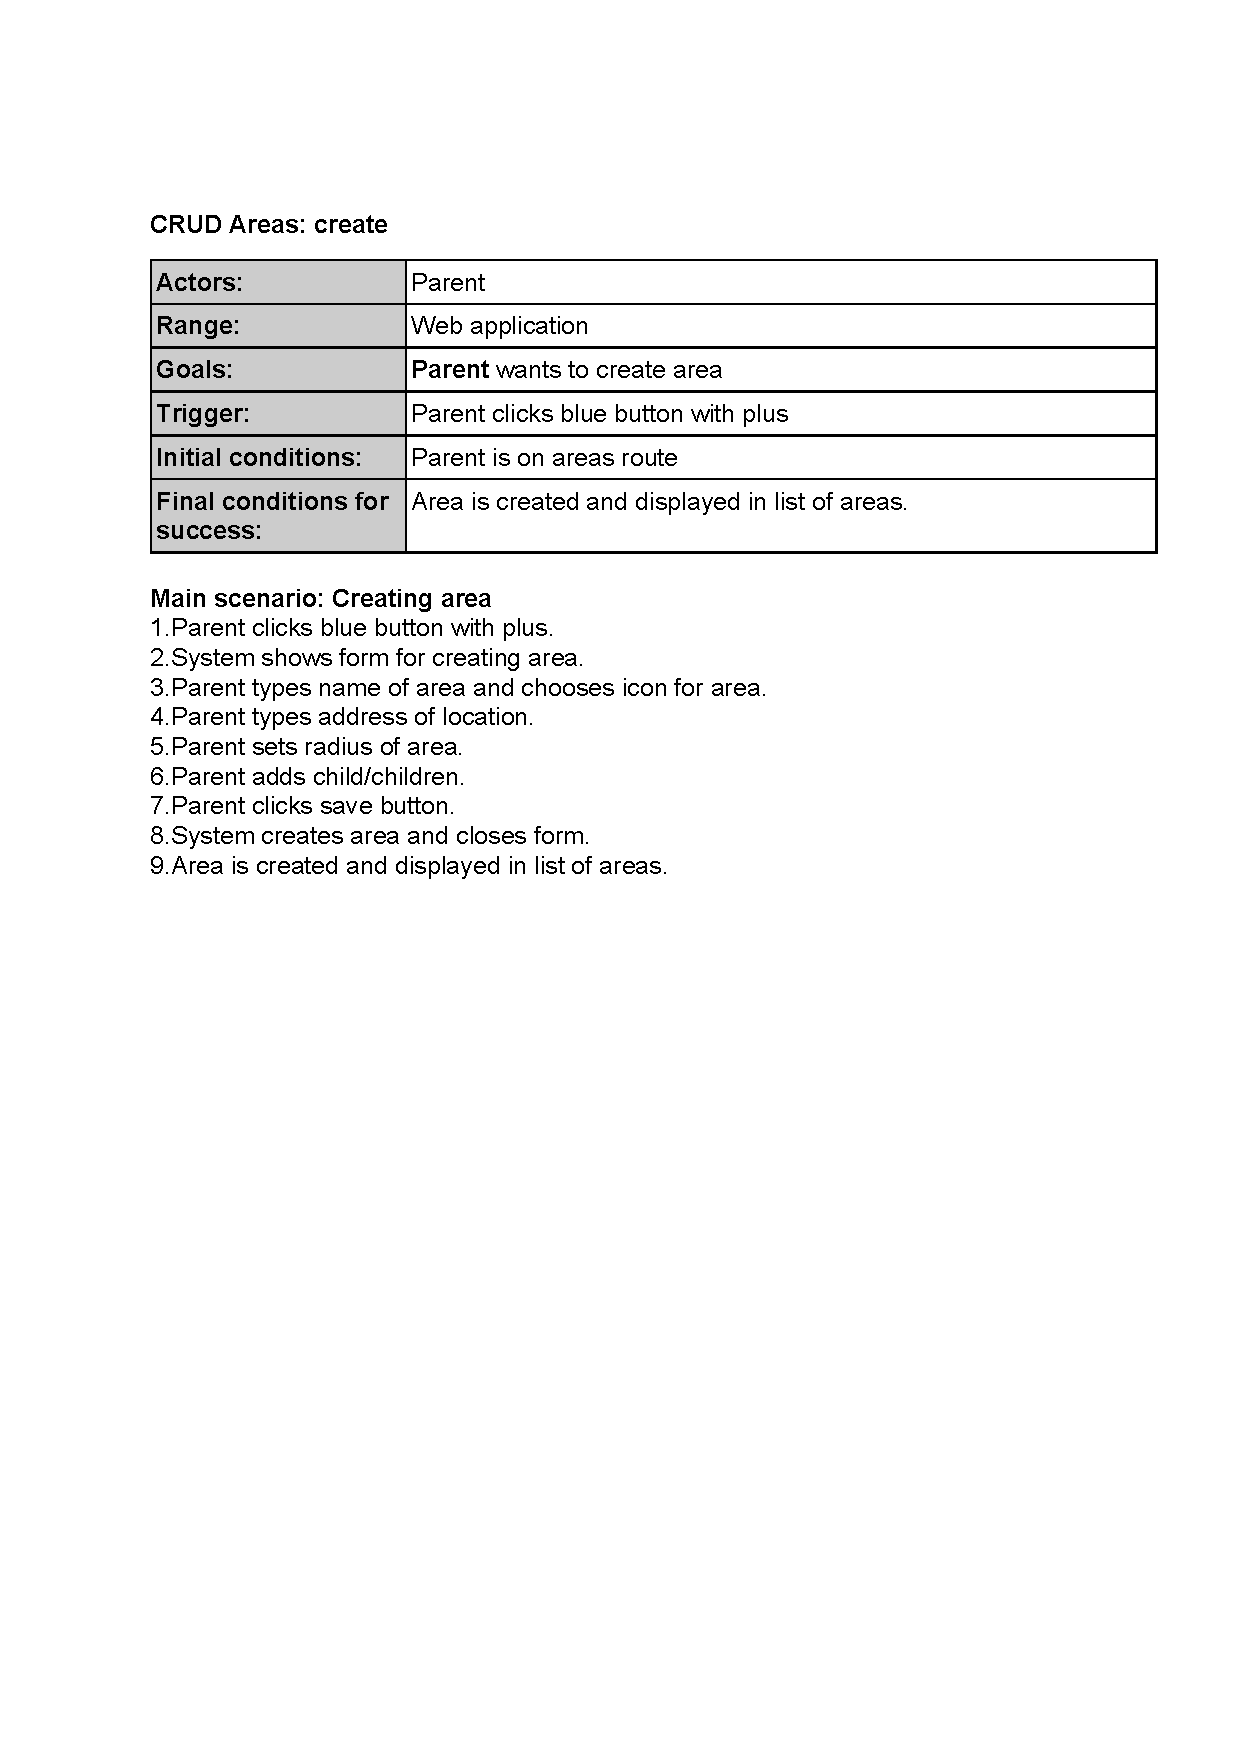
\includegraphics[width=.80\textwidth]{crA_cropped}
    		\end{tabular}
    		\caption{Creating area scenario}
    	\end{figure}

    	\begin{figure}[H]
    		\centering
    		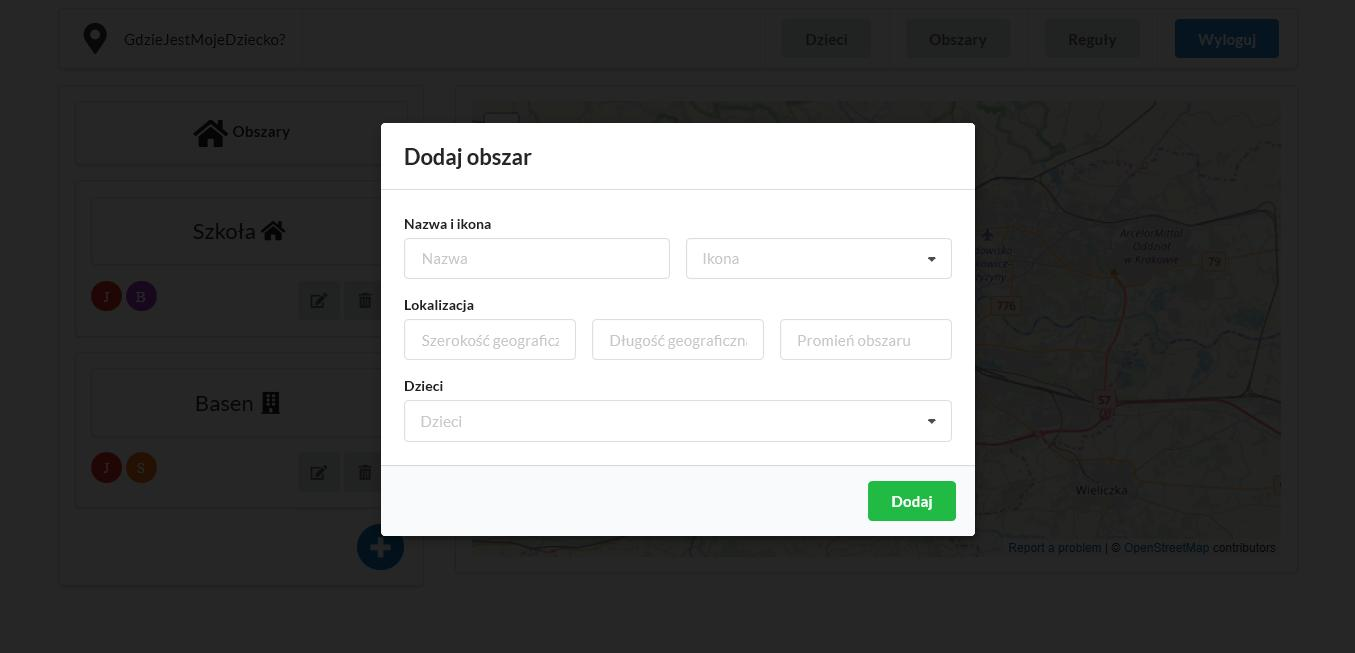
\includegraphics[width=.80\textwidth]{addArea}
    		\caption{Creating area}
    	\end{figure}

    	\begin{figure}[H]
    		\centering
    		\begin{tabular}{c}
    			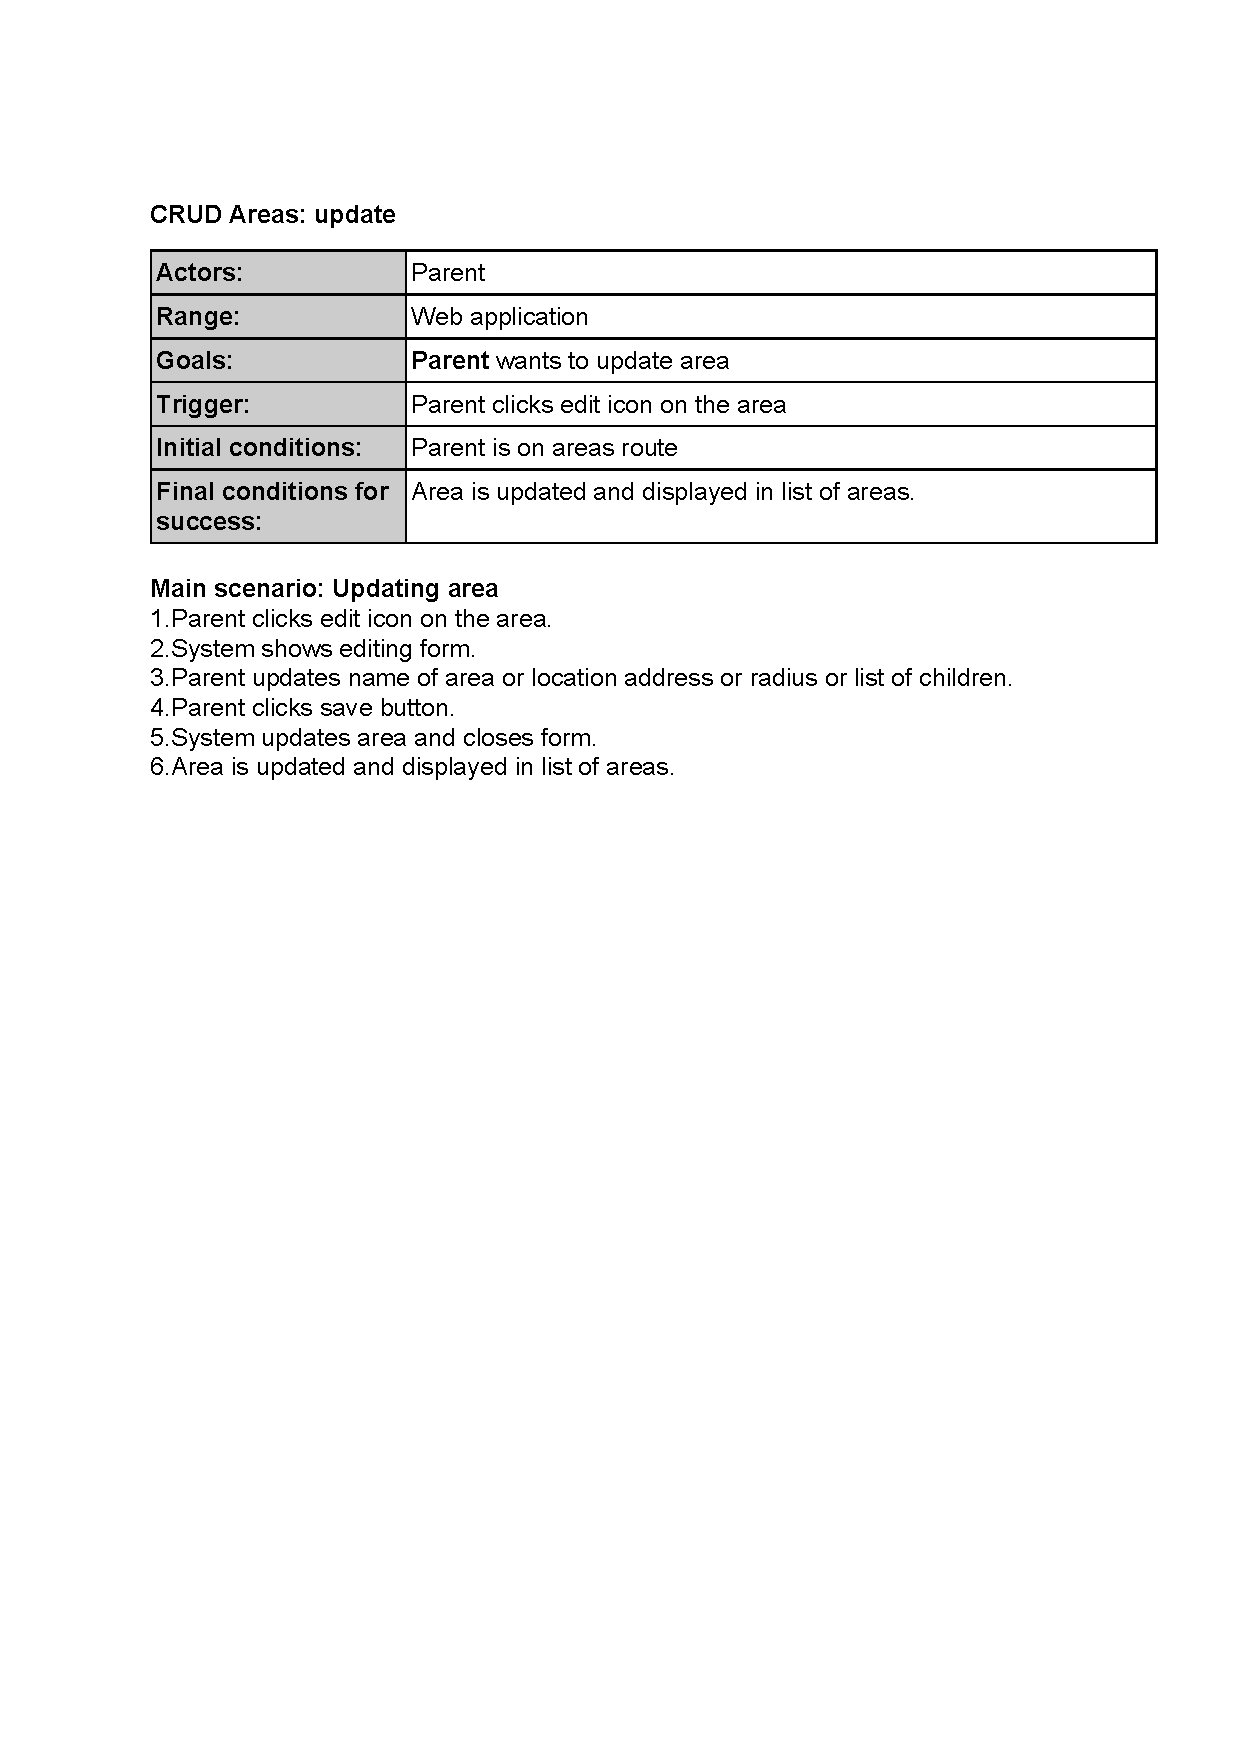
\includegraphics[width=.80\textwidth]{upA_cropped}
    		\end{tabular}
    		\caption{Updating area scenario}
    	\end{figure}

    	\begin{figure}[H]
    		\centering
    		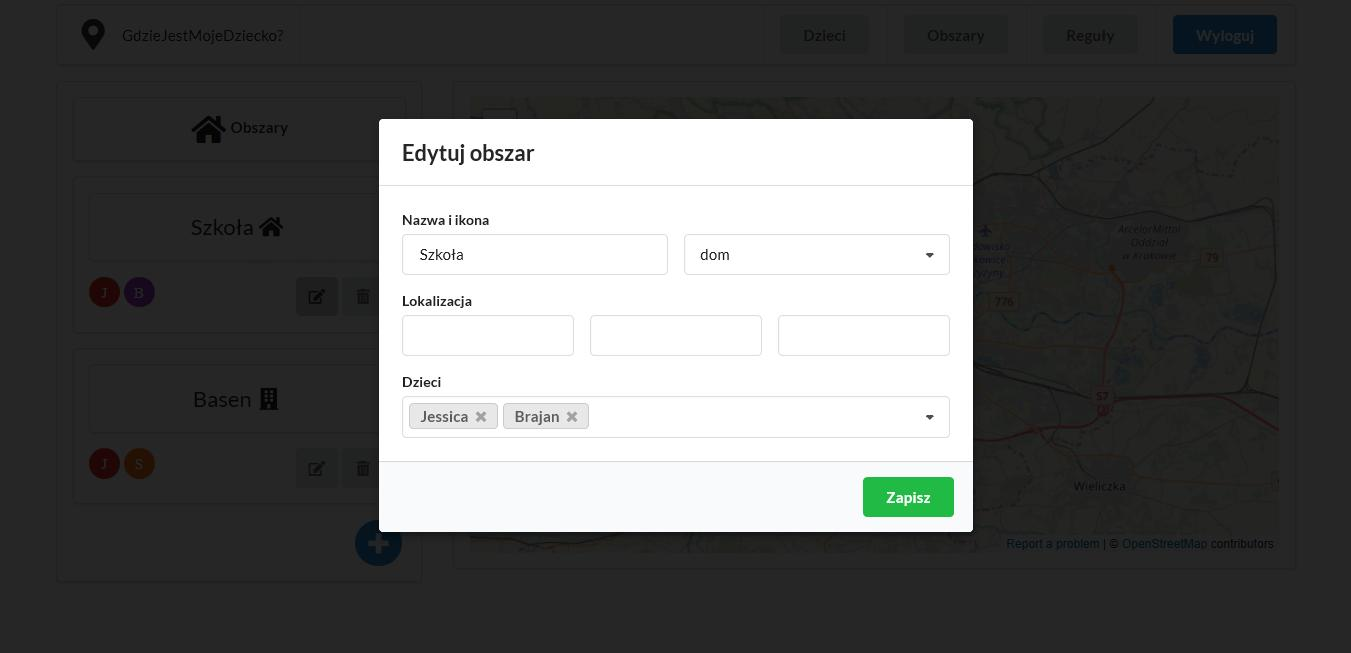
\includegraphics[width=.80\textwidth]{editArea}
    		\caption{Editing area}
    	\end{figure}

    	\begin{figure}[H]
    		\centering
    		\begin{tabular}{c}
    			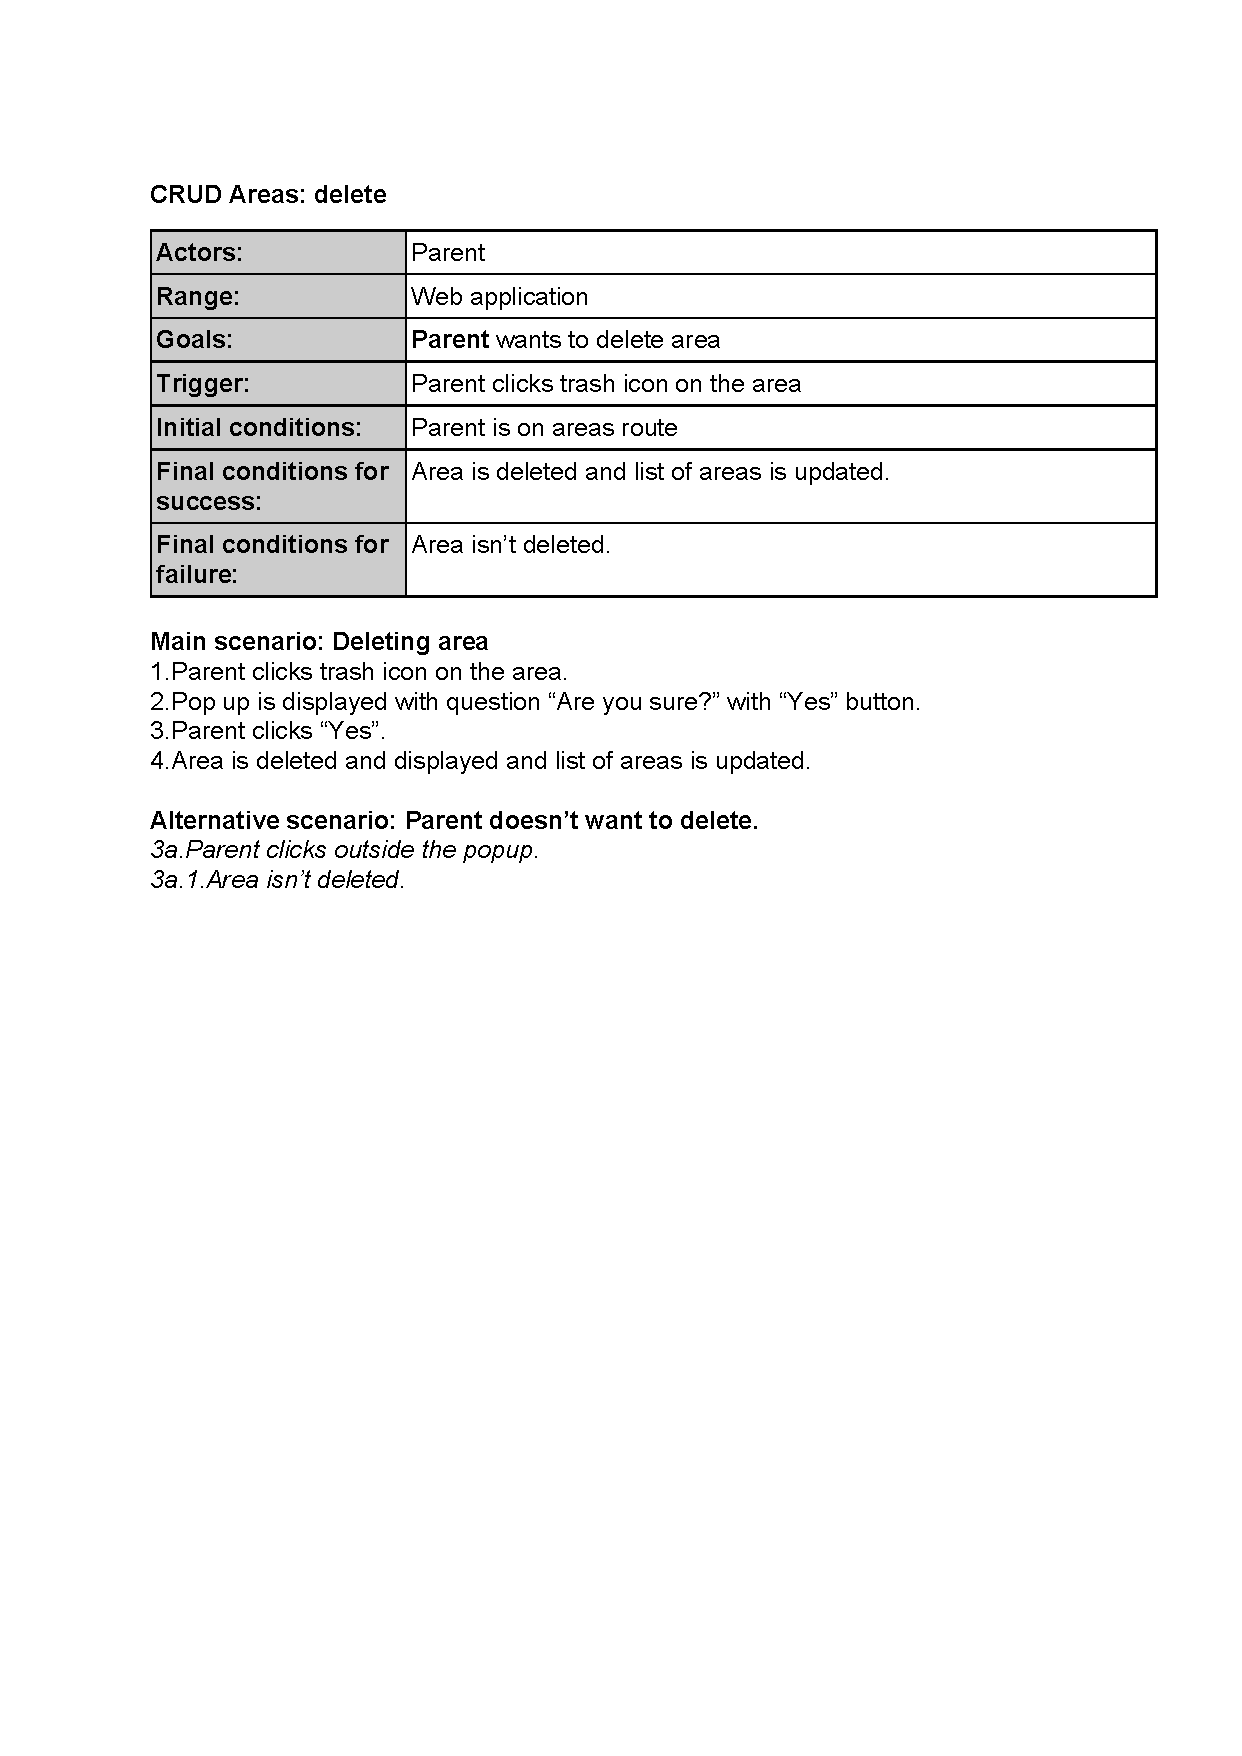
\includegraphics[width=.80\textwidth]{deA_cropped}
    		\end{tabular}
    		\caption{Deleting area scenario}
    	\end{figure}

    	\begin{figure}[H]
    		\centering
    		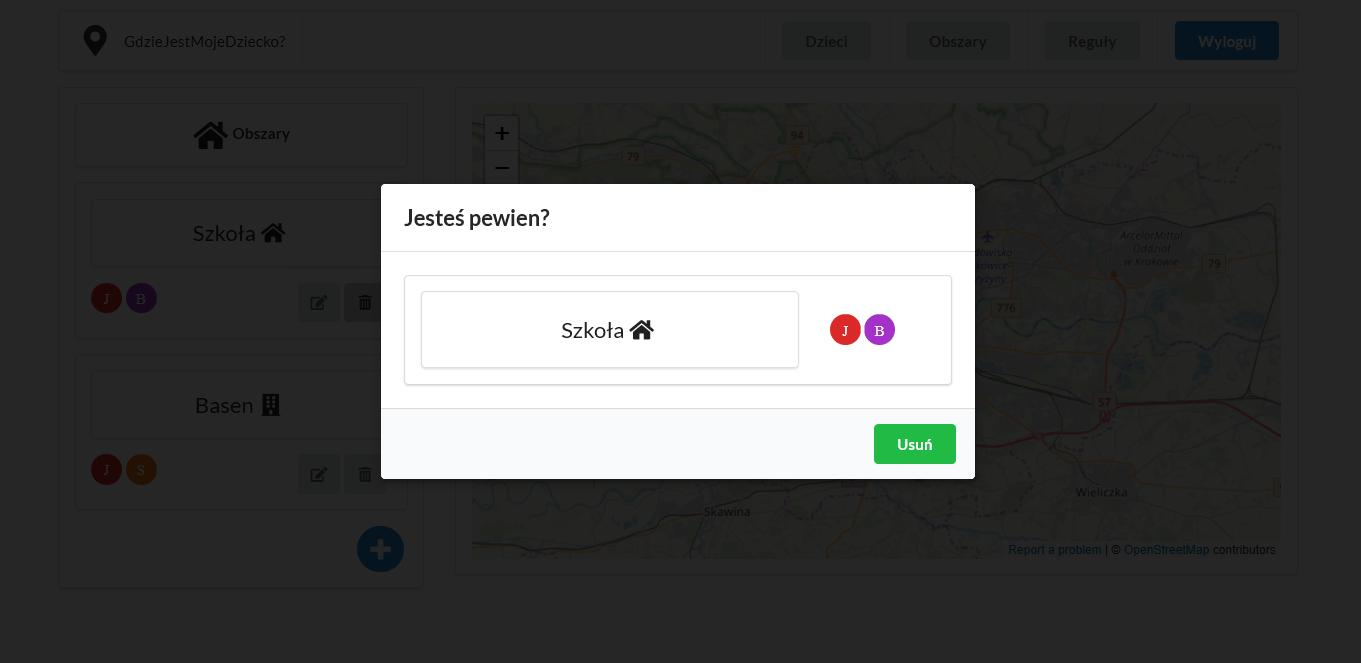
\includegraphics[width=.80\textwidth]{deleteArea}
    		\caption{Deleting area}
    	\end{figure}

    	\begin{figure}[H]
    		\centering
    		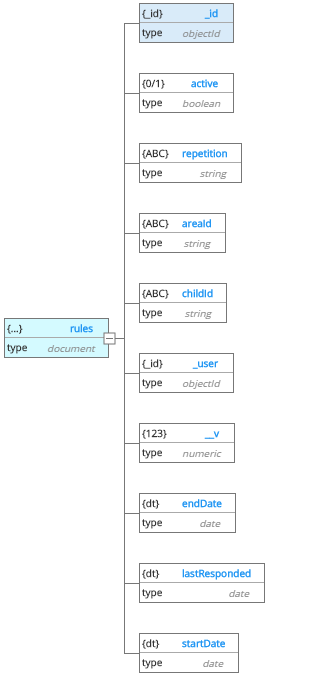
\includegraphics[width=.80\textwidth]{rules}
    		\caption{Rules}
    	\end{figure}

    	\begin{figure}[H]
    		\centering
    		\begin{tabular}{c}
    			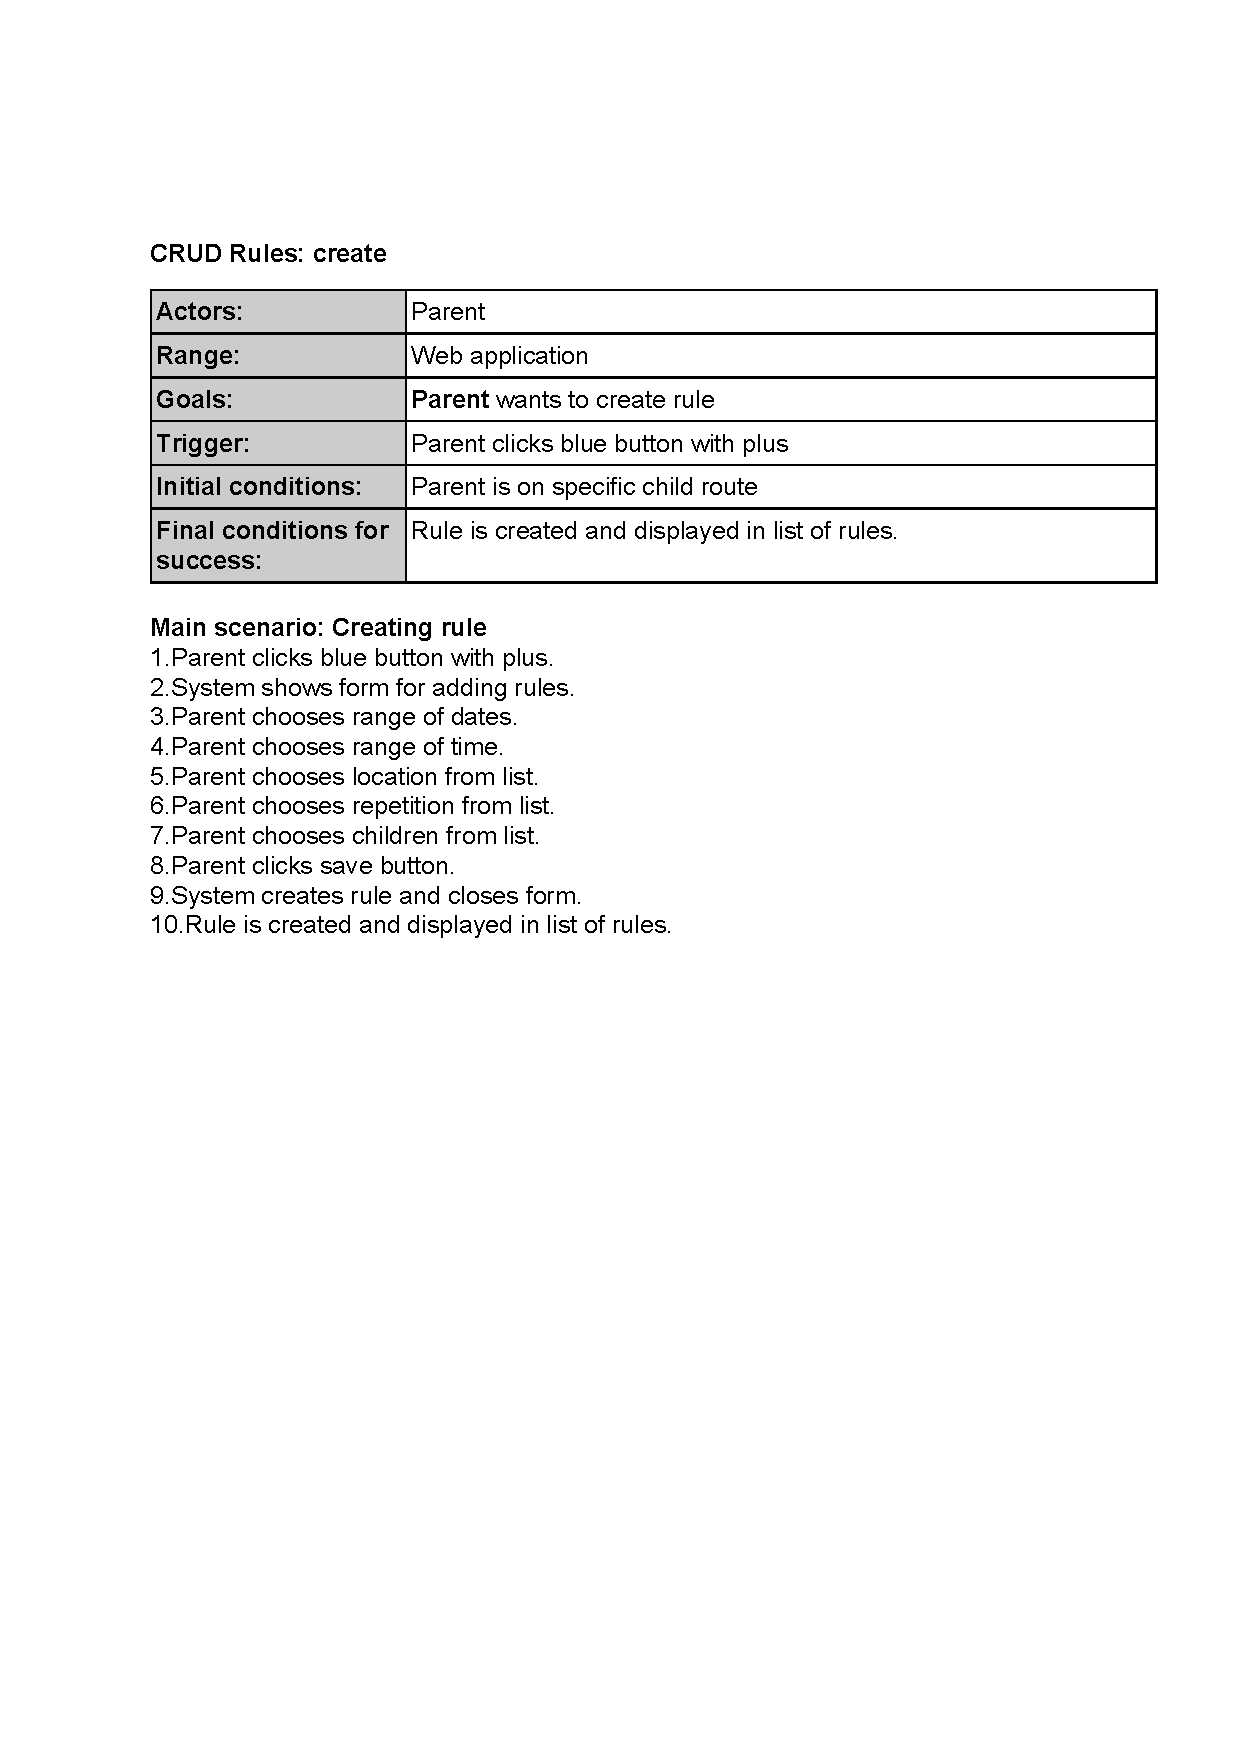
\includegraphics[width=.80\textwidth]{crR_cropped}
    		\end{tabular}
    		\caption{Creating rule scenario}
    	\end{figure}

    	\begin{figure}[H]
    		\centering
    		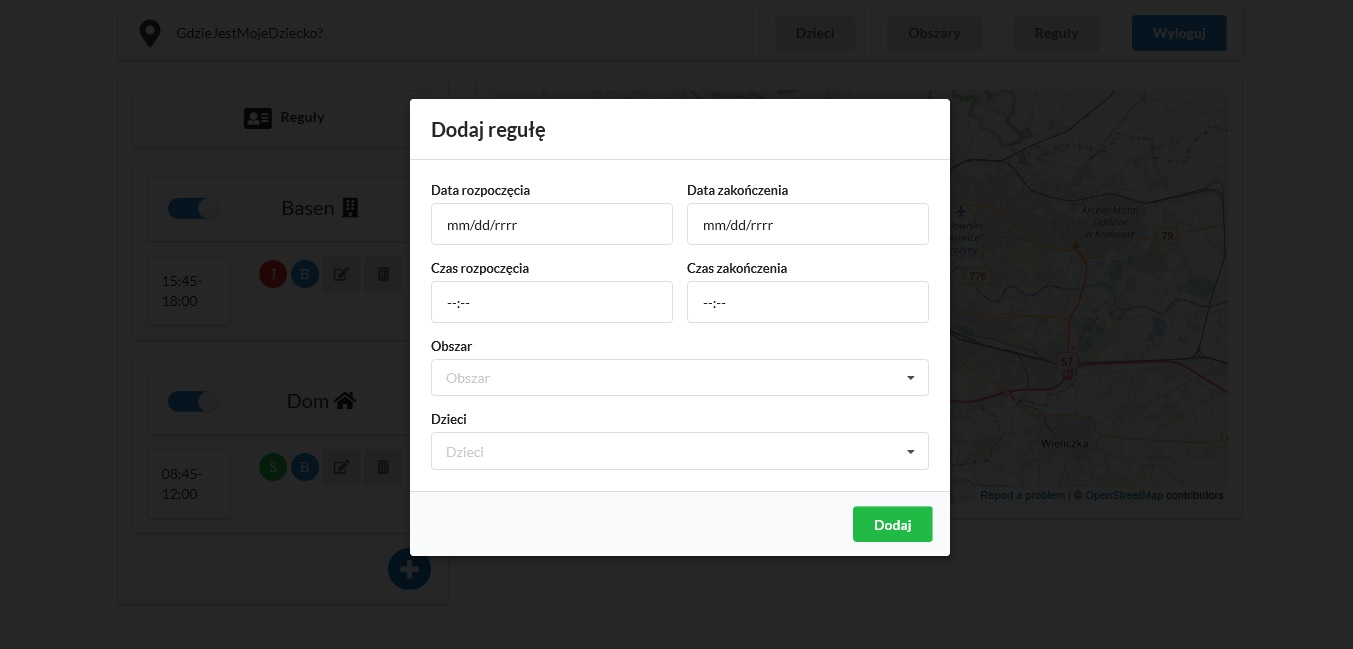
\includegraphics[width=.80\textwidth]{addRule}
    		\caption{Creating rule}
    	\end{figure}

    	\begin{figure}[H]
    		\centering
    		\begin{tabular}{c}
    			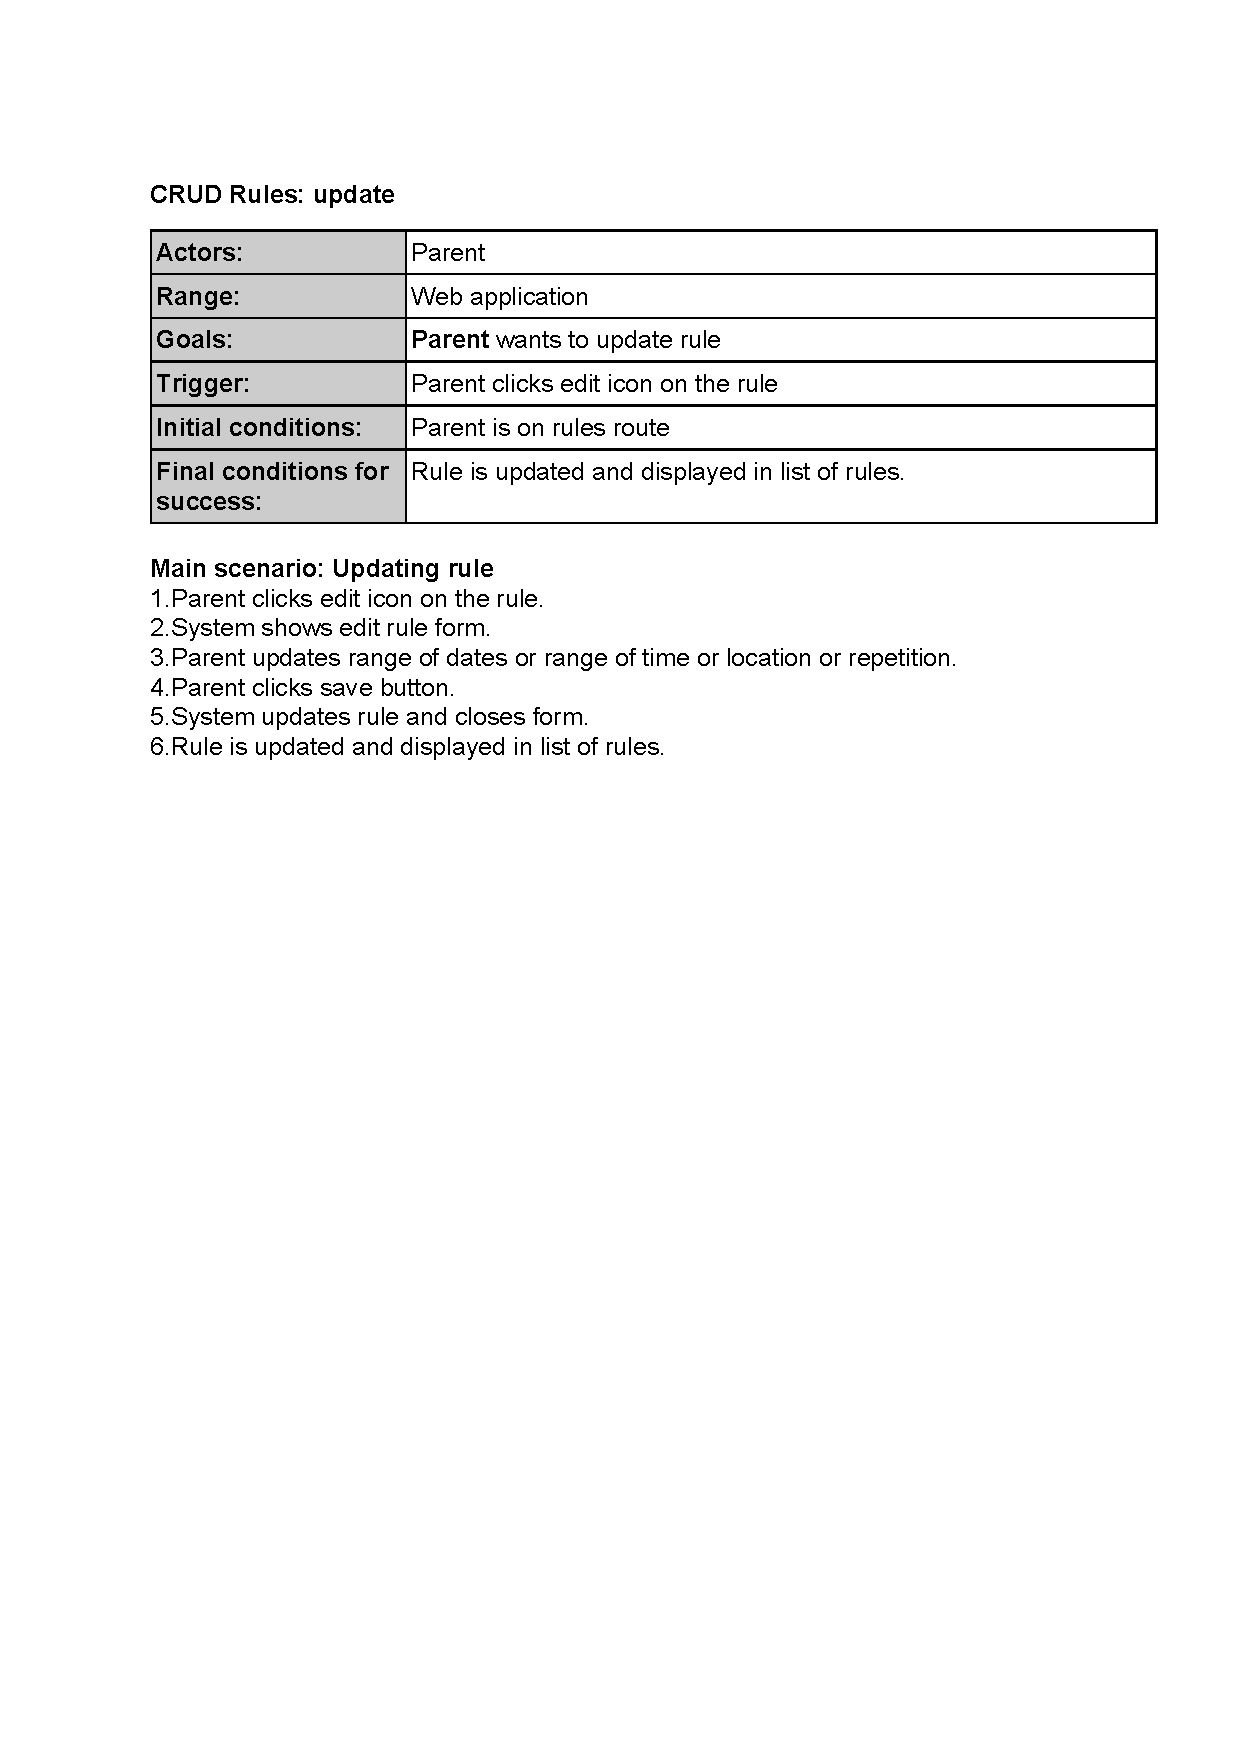
\includegraphics[width=.80\textwidth]{upR_cropped}
    		\end{tabular}
    		\caption{Updating rule scenario}
    	\end{figure}

    	\begin{figure}[H]
    		\centering
    		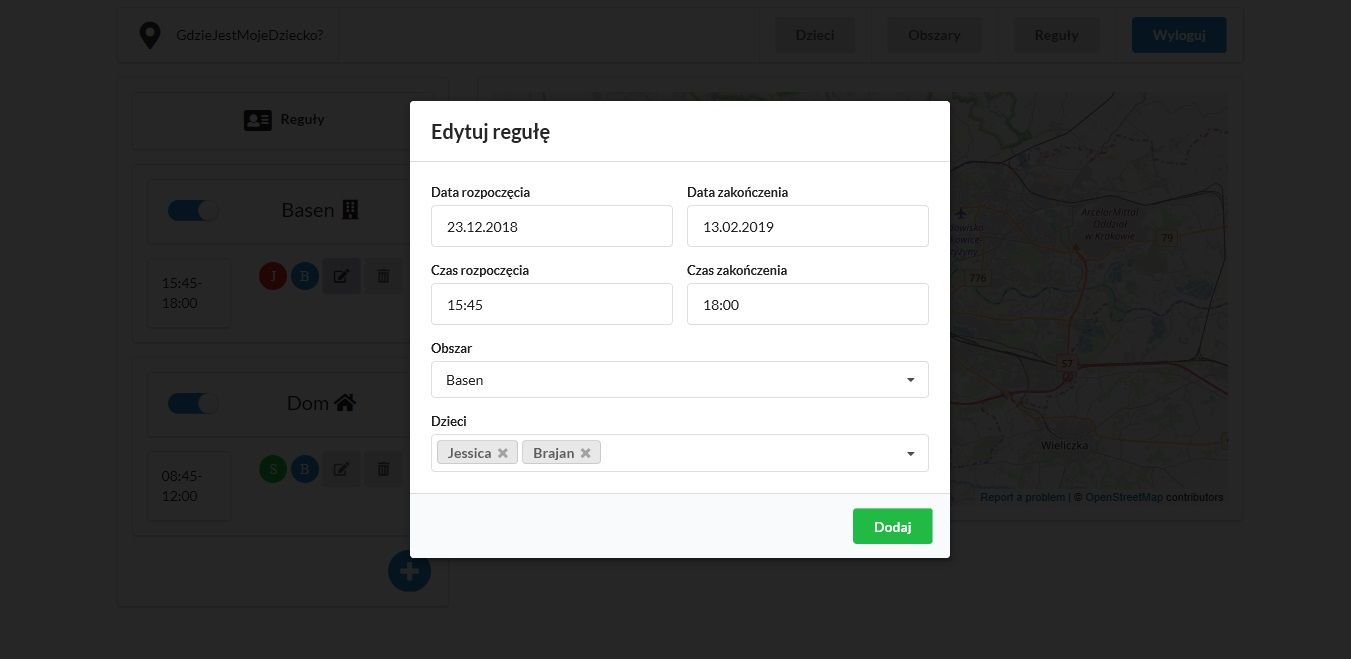
\includegraphics[width=.80\textwidth]{editRule}
    		\caption{Updating rule}
    	\end{figure}

    	\begin{figure}[H]
    		\centering
    		\begin{tabular}{c}
    			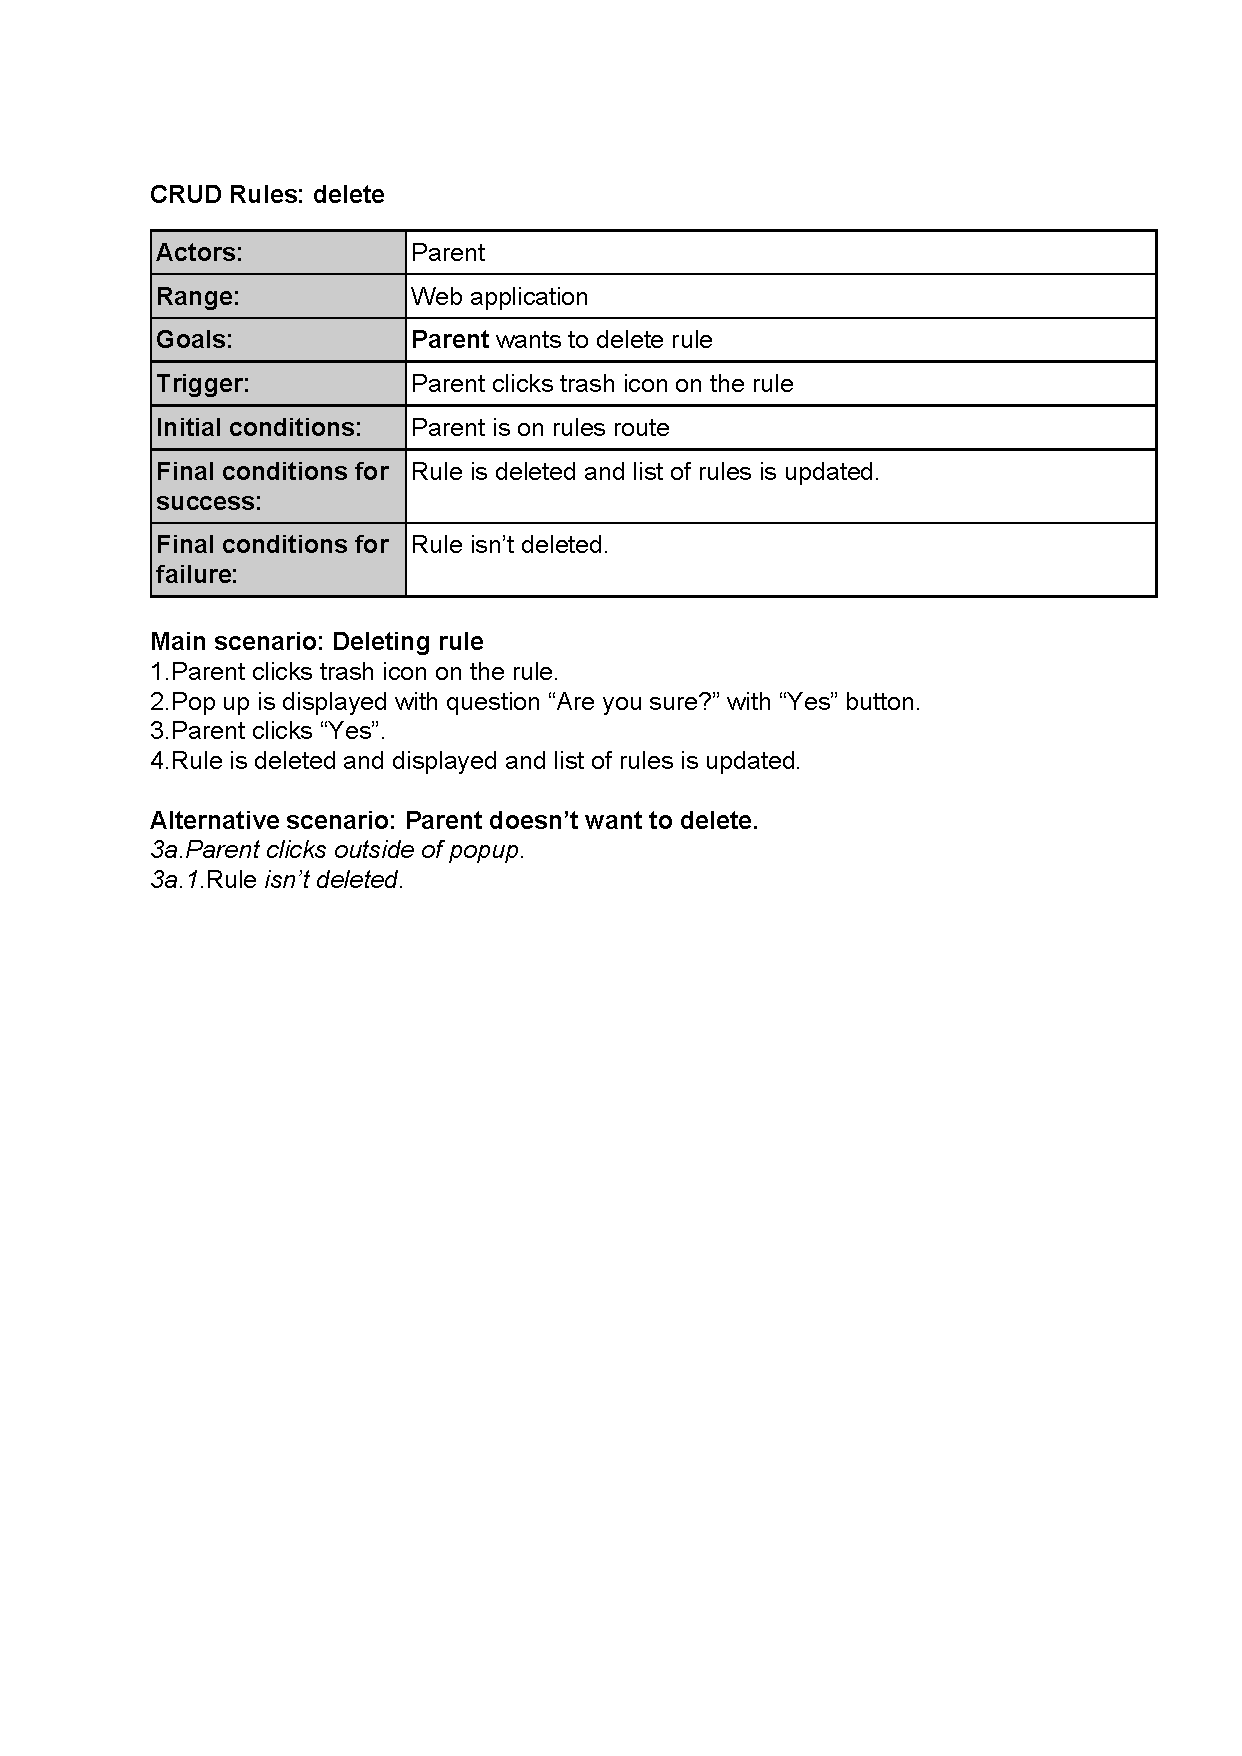
\includegraphics[width=.80\textwidth]{deR_cropped}
    		\end{tabular}
    		\caption{Deleting rule scenario}
    	\end{figure}

    	\begin{figure}[H]
    		\centering
    		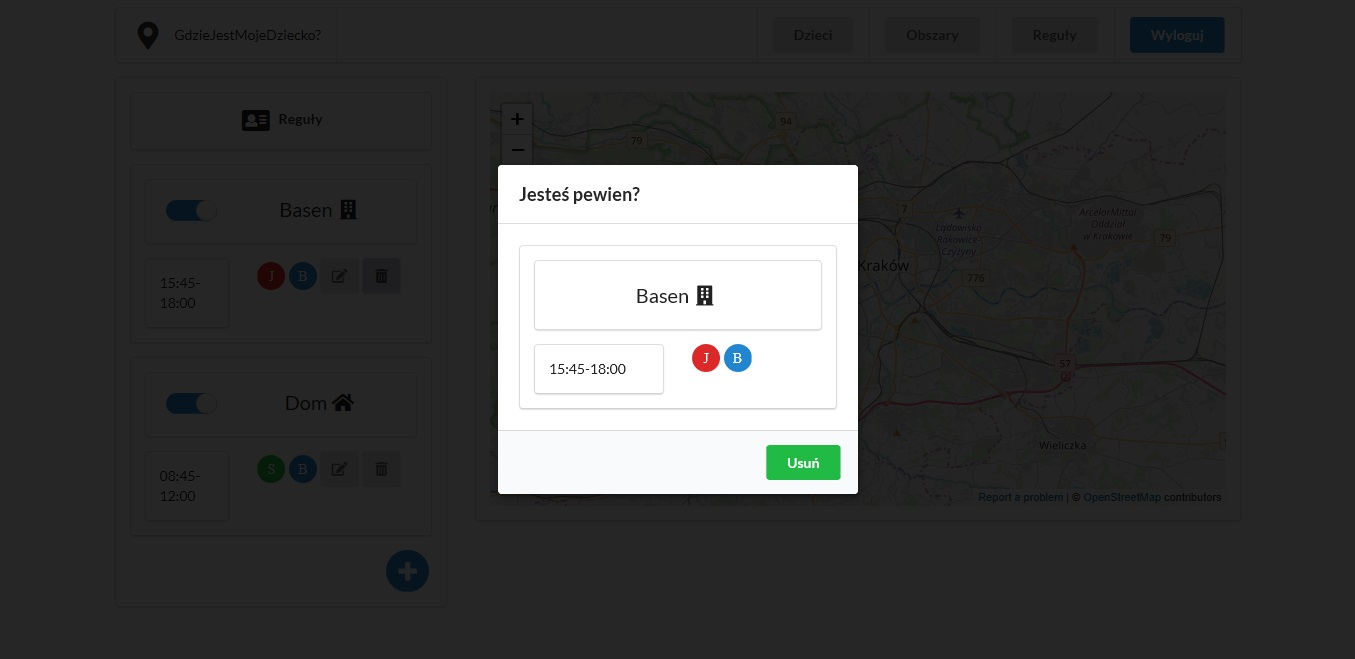
\includegraphics[width=.80\textwidth]{deleteRule}
    		\caption{Deleting rule}
    	\end{figure}

\end{document}